\documentclass[a4paperm]{article}
%\documentclass[12pt,twocolumn]{article}

\usepackage[T2A]{fontenc}
\usepackage[utf8]{inputenc}
\usepackage[russian,english]{babel}
\usepackage{amsmath,amsthm,amssymb,stackrel}
\usepackage[affil-it]{authblk}
\usepackage{cite}
\usepackage{scrextend}
\usepackage{verbatim}
\usepackage{paralist}
\usepackage[mediumspace,mediumqspace,Grey,squaren]{SIunits}
\addtokomafont{labelinglabel}{\sffamily}
\usepackage{amsmath}
\usepackage{graphicx}
 \usepackage[usenames, dvipsnames]{color}
 \usepackage{multirow}
 \usepackage{longtable}
 \usepackage{lineno}
 \usepackage{textcomp}
 
 \usepackage{xr}
 \usepackage{longtable}
 \usepackage{array} 
 
%\usepackage[none]{hyphenat} %no nyphenation

\usepackage{SIunits}
\usepackage{miller}
\usepackage[version=3]{mhchem}

\usepackage{float} %H with figures

\setlength{\parindent}{5ex}

 \usepackage{newfloat} %For numbering of supplemmentary figures
 \DeclareFloatingEnvironment[name={Supplementary Figure}]{suppfigure}

\graphicspath{{figures/}}
\externaldocument{SI/smose_supp}

\usepackage[outdir=./]{epstopdf}



\begin{document}

%\linenumbers

\title{Janus structures of SMoSe and SVSe compositions with low enthalpy and unusual crystallchemistry}


\author[1,2,3]{Pavel N. Gavryushkin
   \thanks{Electronic address: \texttt{gavryushkin@igm.nsc.ru, p.gavryushkin@g.nsu.ru}; Corresponding author}}     
\author[2]{Nursultan Sagatov}
\author[1]{Ekaterina V. Sukhanova}
\author[1]{Zakhar I. Popov}
\author[4]{Inna Medrish}

\affil[1]{Emanuel Institute of Biochemical Physics of Russian Academy of Sciences, 4 Kosygin Street, Moscow, 119334, Russian Federation}
\affil[2]{Sobolev Institute of Geology and Mineralogy, Siberian Branch of Russian Academy of Sciences, prosp. acad. Koptyuga 3, 630090 Novosibirsk, Russian Federation}
\affil[3]{Novosibirsk State University, Pirogova 2, Novosibirsk 630090, Russian Federation}
\affil[4]{Samara Center for Theoretical Material Science (SCTMS), Samara State Technical University, Molodogvardeyskaya St. 244, Samara, Russia 443100}


\date{}
\maketitle

%\linenumbers

\begin{abstract}
Transition metal dichalcogenides (TMDs) like MoS$_2$ or WS$_2$ together with graphene and \textcolor{red}{its derivatives are the most perspective and widely investigated 2D structures (Захар замени это более конкретной фразой)}.
TMDs with top and bottom layers consisting of sulfur and selenium atoms, respectively, were produced experimentally and were called Janus structures.
Here, we perform the theoretical search of the new Janus structures with compositions SMoSe and SVSe.
Two crystal structures, 1M-SVSe and 1A'-SMoSe are especially promising for experimental synthesis and practical applications.
These structures are dynamically stable and the enthalpy of 1M-SVSe is 0.22 ev/f.u. lower than that of 1T-SVSe, while the enthalpy of 1A'-SMoSe is 0.12 ev/f.u. lower than the enthalpy of 1T-SMoSe.
The presence of the vanadium atoms having magnetic moment in the 1M-SVSe crystal structure implies it's possible application as \textcolor{red}{magnetic material (Захар, уточни здесь])}.
In the work, we perform the detailed crystall-chemical analysis of the predicted structures and show that some of the dynamically stable structures are characterised by the unique for TMDs crystall-chemical features, among which are quadruple Mo--Mo bonds and covalent S--S, Se--Se bonds.
We also illustrate the tendency of Mo-bearing TMDs to the formation of strong Mo--Mo bonds with chains or isolated  dimers of molybdenum atoms.
This feature is not characteristic of vanadium-bearing TMDs.

\end{abstract}


\section*{Phase renaming}
fes = 1S \\
fxt = 1H' \\
T-hor-SVSe = 1M-SVSe \\
H-hor-SMoSe = 1M'-SMoSe \\
SVSe-airss1 = 1A-SVSe \\
SMoSe-airss1 = 1A'-SMoSe \\
SVSe-airss3 = 1A''-SVSe \\
SMoSe-airss3 = 1A'''-SMoSe \\
test1 (SMoSe) = 1O \\
test2 (SMoSe) = 1O' \\
test3 (SMoSe) = 1M'' \\


%%%%%%%%%%%%%%%%%%%%%%%%%%%%%%%%%%%%%
\section{Introduction}
%%%%%%%%%%%%%%%%%%%%%%%%%%%%%%%%%%%%%

Transition metal dichalcogenides (TMDs) represent a wide family of materials consisting of transition metal (TM) of group IV--VI surrounded by chalcogen atoms (Ch) of S, Se, or Te. 
TMDs crystallize in four main structural types, CdI$_2$, MoS$_2$ and FeS$_2$-pyrite, and less frequently -- in FeS$_2$-marcasite structural type \cite{wells}.

The first two structural types are characterized by the layered structures with Ch-TM-Ch sandwiches bonded with each other by the weak Van-der-Waals bonds and, therefore, the crystals can be exfoliated into individual stable layers \cite{zhang2020intercalation}. These quasi-2D sandwiches attract considerable attention due to their wide range of properties \cite{li2017graphene, SHI20181, xi2016ising, hu2019recent, pi2019recent}. 
Particularly the TMDCs can act as semiconductors \cite{nayeri2018transport}, metals \cite{zhao20212d}, semimetals \cite{xu2020high, zhao2020observation} or superconductors \cite{wang2020nodeless,hsu2017topological} which make family of TMDs suitable for a lot of applications. 

At ambient conditions MX$_2$ (M=Mo,W, X=S,Se) structures crystallize in the archetype molybdenite structure (MoS$_2$) which consists of close-packed layers of chalcogen atoms placed exactly one under/above another and TM atoms occupy one half of the  trigonal prismatic cavities located between the layers of chalcogen atoms. 
In the most stable polytype of molybdenite (MoS$_2$) structure M--X--M multiplet layers are arranged similarly to the close-packed layers of {\it hcp} structure -- close-packed structure with periodicity of stacking through each two layers, the structure (Figure \ref{1H1T}a).
Due to hexagonal symmetry this structure of TMD according to Ramsdell notation can be denoted as 2H.
In the present work, we do not consider the stacking sequence of M--X--M sandwich and will denote all structures as 1H.
Such a sandwich, consisting of three layers, in crystalchemical community usually termed as {\it multiplet layer}.
However in 2D community the term {\it monolayer}, emphasising absence of van-der-waals bonds wihtin the layer, is more accepted and we will follow the last tradition. 

If one layer of chalcogen atoms in M--X--M monolayer is shifted, the coordination polyhedron of metal atoms is changed from trigonal prism to the octahedron (Figure \ref{1H1T}b).
This is CdI$_2$ structural type. 
The monolayer of such a structure has trigonal symmetry and can be designated as 1T \cite{huang2020recent}. 
The deformed 1T structure with chains of Mo atoms connected by the shorted bonds is denoted as 1T' \cite{huang2020recent}.
Depending on the exact chemical composition of the TMD monolayer, 1H or 1T phase is thermodynamically stable \cite{ataca2012stable}. 
For the disulphides, diselenides, and ditellurides of Mo or W, the  1T-phase is less energetically favorable than 1H-phase with the same chemical composition. 
However 1T structure can be obtained by means of intercalation \cite{kan2014structures, wang2014atomic}, deformation \cite{duerloo2014structural} or surface functionalization \cite{tang2015stabilization, voiry2015covalent}. 
In contrast to Mo, W and most of the other TMs, dichalcogenides of vanadium are not known \cite{murphy1977preparation, le1979elaboration}. 
Only Se$_2$V$1.005$ with additional vanadium atoms located in the centers of empty trigonal prismatic cavities is known in the form of 2H structure \cite{rigoult1982}.

Recently a new subclass of TMDs where top and bottom layers are formed by different chalcogen atoms, were produced and attracts significant interest \cite{lu2017, zhang2017janus}. 
Such a structures were called called Janus structures.
The opportunity to change the top layer of atoms opens an additional degree of freedom to manipulate the properties of TMDs. 
Janus TMDs have structural symmetry breaking \cite{li2017electronic, van2020first} resulting in Rashba spin splitting \cite{hu2018intrinsic} and transverse dipole moment leading to large piezoelectricity \cite{dong2017large, li2018recent}. 
The Janus structures of TMDs have a lot of potential applications, among which water-splitting \cite{xia2018universality, ma2018janus} or hydrogen evolution reaction \cite{er2018prediction, zhou2019janus}. 
Theoretical investigations show that, as in the case of pristine monolayers, Janus TMDs with different chemical compositions can be thermodynamically stable in the 1H and 1T structures desrcibed above.
Meanwhile, the different composition of the top and bottom layers assume the possibility for the stabilization of the new structures, substantially different from 1H or 1T.

This assumption was the motivation for us to perform the search for the new Janus TMDs structure using unbiased methods of crystal structure prediction, which have not been performed jet.




\begin{figure}[H]
        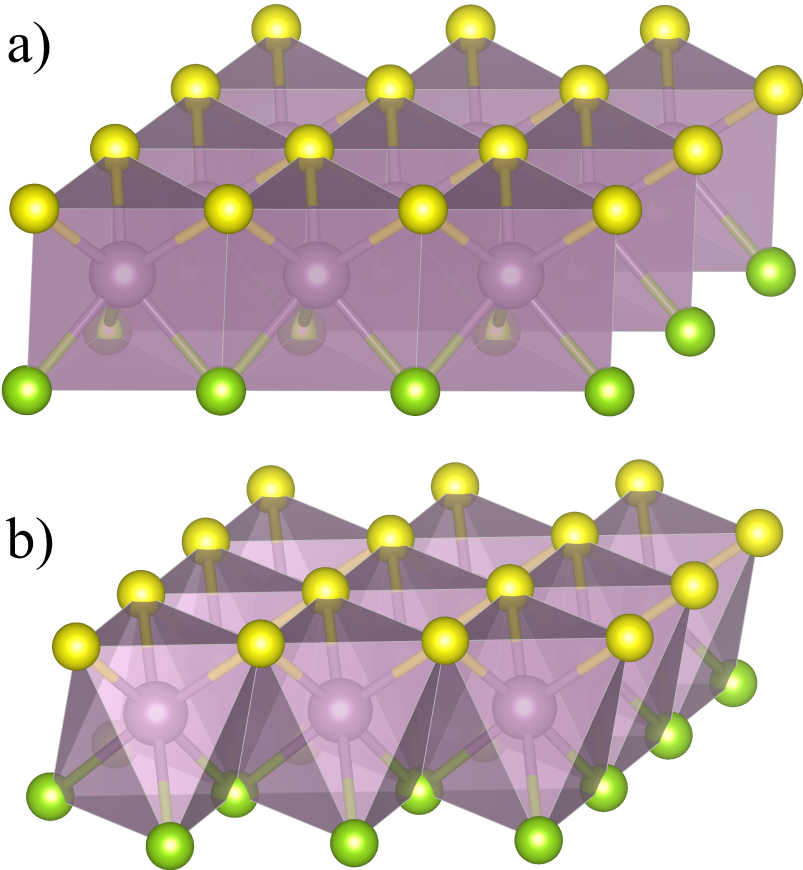
\includegraphics[width=0.4\textwidth]{1H1T.png}
        \caption{Packing of trigonal prisms and octahedra in 1H (a) and 1T (b) structures of SMoSe.}
\label{1H1T}
\end{figure}





%%%%%%%%%%%%%%%%%%%%%%%%%%%%%%%%%%%%%
		\section{Methods}
%%%%%%%%%%%%%%%%%%%%%%%%%%%%%%%%%%%%%

%%%%%%%%%
\subsection*{Crystal structure prediction}
%%%%%%%%%


The search for the lowest-enthalpy monolayer structures of SMoSe and SVSe compositions was performed using evolutionary algorithms implemented in the USPEX program package \cite{uspex1,uspex2,uspex3} and the random sampling method implemented in the AIRSS software \cite{airss1,airss2}.

The crystal structure search within USPEX was performed in fixed composition mode with 2--6 formula units per unit cell.
The number of structures in the first generation of the calculations was equal to 180.
Half of the structures with the lowest enthalpy were selected after the optimization and then used to produce the next generation.
A new generation was produced as follow: 50\% of all structures were generated by heredity, 10\% -- by atomic mutation, 10\% –- by lattice mutation, and 30\% –- randomly.
In average, 40--47 generations were produced and relaxed.
Using AIRSS program about 5000--6000 structures were randomly generated and optimized for compounds with 4 and 6 formula units per unit cell and structures with the lowest enthalpy were selected.

The total energies and forces were calculated by solving the Schr\"{o}dinger equation based on projector augmented plane-wave implementation \cite{blochl1994projector} of density functional theory (DFT) using the VASP program package \cite{vasp1,vasp2}.
Exchange correlation effects were treated in the generalized gradient approximation (GGA) with Perdew-B\"{u}rke-Ernzerhof scheme \cite{pbe}.

In all crystal structure prediction calculations medium-quality optimization was performed using the conjugate gradient method \cite{conjugate_gradient}. 
The energy cutoff of plane waves was set to 420 eV and 700 eV for the intermediate structures and then for the most promising of them. 
The first Brillouin zone was sampled according to Monkhorst-Pack scheme \cite{monkhorst1976special} with the density of k-point being equal to 0.5 \AA$^{-1}$ and 0.2 \AA$^{-1}$, respectively. 
% проверить 2pi

To study a dynamic stability of predicted structures phonon dispersion spectra were calculated within the PHONOPY code \cite{phonopy}. 
We used VESTA program for crystal structures visualization and figures preparation \cite{momma2011vesta}.
Instruments of Bilbao Crystallographic server have been used for the structures symmetrisation \cite{bilbao}.


%%%%%%%%
\subsection*{Topological search}
%%%%%%%%

Within topological search, original crystal-structural information was selected from the Inorganic Crystal Structure Database (ICSD, release 2020/2) \cite{icsd_1} and Cambridge Structural Database (CSD, release 2021) \cite{icsd_2}.
In this case, the procedures of screening of structural-graphic databases of compounds by the methods of the combined geometric-topological analysis with ToposPro (http://topospro.com) package have been used \cite{topos_1}. 

We use bold three-letter symbols of the Reticular Chemistry Structure Resource nomenclature (for the three-letter nomenclature of polyhedral and nets see Reticular Chemistry Structure Resource, http://rcsr.anu.edu.au/, and \cite{rcsr}) or ToposPro NDk-n symbols \cite{rcsr_2}) to designate the topological types of the underlying nets. 
The topology of an underlying net is determined in an automated mode by comparison of a set of topological indices of the net with those for the reference nets from the ToposPro TTD collection \cite{TTD}.

For the topological analysis we have used only fully solved crystal structures without errors in the determination of interatomic bonds or chemical composition,
The nets of interatomic bonds were determined by the Domains methods with the program AutoCN \cite{blatov2016_rods}. 
Only strong interatomic bonds  with solid angles of the faces of Voronoi-Dirihle polyhedron $\Omega \geq 5 $ of the whole 4$\pi$ solid angle were considered.
Structures with the great values of unit cell parameters were excluded from the consideration.
For instance, we did not consider polytypes of ZnS with cell parameters more than 50 \AA.

Earlier the numerous structural relations between unhydrous simple salts and even more simple binary inorganic compounds have been shown \cite{blatov2011_salts, medrish2020_zintl}. 
Due to this well-known structural phenomena, we analyse topology not only for the complete  representation, but all so the topology of the underlying net.
In the complete representation, the net corresponds to the interatomic bonds of all strong bonds, while the underlying net is determined between metals and centers of ligands.

Due to the short interatomic bonds, the topologies were not determined for the crystal structures airss1, 1H', and  1M''.


%%%%%%%%%%%%%%%%%%%%%%%%%%%%%%%%%%%%%
			\section{Results}
%%%%%%%%%%%%%%%%%%%%%%%%%%%%%%%%%%%%%

\subsection*{Earlier known MX$_2$ structures and their enthalpies}

Although 1H and 1T structures are characterized by the different coordination polyhedra, they are similar in the manner of their interconnection.
The H structure consists of trigonal prisms [MX$_6$], and 1T structure –- of the [MX6] octahedra, where X is chalcogen atom of sulfur or selenium (Figure\ref{1H1T}).
Each trigonal prism share all three vertical edges with the neighbouring prisms and does not share any faces (Figure \ref{1H1T}a).
As the result, each vertex and each vertical edge of the trigonal prism is common for three prisms (Figure \ref{1H1T}a).
Similarly in 1T structure, each octahedron share all edges inclined to the plane of sulfur atoms with neighbouring octahedra, and each vertex is common for three octahedra (Figure \ref{1H1T}b).
Bond valence of Mo--S bond is nearly equal to +4/6 and there are necessary three such a bonds to compensate negative charge of S$^{2-}$.
Interconnection through the faces gives shorter bonds between high-charged M$^{4+}$ ions, increasing the energy of Couloumb interaction, and making the structure less favourable \cite{pauling1929}.
As we will shown below the interconnection through the faces is also realized for predicted structures, but they are less favourable than 1H or 1T structure.

According to the performed calculations, 1H structure is the most favourable for SMoSe composition, but it is less favourable than 1T and 1T' for SVSe composition.
The difference of enthalpies $H(1H)-H(1T)$ is equal to -0.73 ev/f.u. for SMoSe and 0.09 for SVSe (Table \ref{t:enthalpy}).
For SVSe composition the most favourable phase is 1T', which enthalpy is 0.11 ev/f.u lower than the enthalpy of 1T (Table \ref{t:enthalpy}). 

The recently found 1S and 1H' \cite{} \textcolor{red}{Захар, поставь ссылку} structures are also characterized by the trigonal prismatic coordination.
However, in these structure prisms are connected not only through edges but also through the faces (Figure \ref{fes_fxt}).
In accordance with above consideration, the enthalpies of 1H' and 1S structures are higher than that of 1H structure, although lower than that of 1T structures.
As well as in 1H and 1T structures, in 1H' and 1S structures,  each chalcogen atoms is connected to three atoms of transition metal, providing the local charge balance (Figure \ref{fes_fxt}).
As we will show below, this is also not the obligatory requirement and some of the revealed structures are not characterized by the local charge balance.
According to our calculations, 1S and 1H' structures are chacterized by the close values of enthalpies.
For both SMoSe and SVSe, 1S is more energetically favourable than 1H', with enthalpies difference equal to 0.01 ev/f.u. for SMoSe and 0.06 ev/f.u. for SVSe (Table \ref{t:enthalpy}).
In turn, enthalpy of SMoSe-1S structure is 0.79 eV/f.u. higher than enthalpy of the 1H structure.
Enthalpy of SVSe-fex is 0.64 higher than that of 1T'.
According to our calculations, the 1H' and 1S structures in the Janus form are less favourable than 1T (Table \ref{t:enthalpy}).

1H and 1T structures provide the most uniform distribution of the chalсogen and transition metal atoms.
Nets of  both transition metal and chalcogen atoms consist of the geometrically equal triangular rings.
Edge-sharing interconnection of trigonal prisms realized in 1H' and 1S structures inevitably results in the appearance of the cavities greater in volume than the cavities of 1H and 1T structures. 
In 1S structure the cavities have the form of the slightly compressed cube (Figure \ref{fes_fxt}a).
The volume of these cavities is almost two times greater than the volume of the cavities in 1H structure (38.8 \AA$^3$ against 17.7 \AA$^3$).
In case of 1H' structure, the volume of hexagonal cavities (Figure \ref{fes_fxt}b is almost 8 times larger than that in 1H structure (137.8 \AA\ against 17.7 \AA$^3$).

In contrast to trigonal prisms, the face-sharing of the octahedra seems to be problematic for quasi 2D structure, as it is results in the deviation from the flat arrangement.
However, as it will be shown below, the dynamically stable quasi-2D structure characterising by the face sharing octahedra was also revealed.



%%%%%%%%%%%%%%%%%%%%%%%%%%%%%%%%%%%%%
		\subsection{New Janus TMD structures}
%%%%%%%%%%%%%%%%%%%%%%%%%%%%%%%%%%%%%

Table \ref{t:enthalpy} shows the values of enthalpies for the most energetically favorable structures among revealed with USPEX and AIRSS.
 Figures \ref{phon_smose} and  \ref{phon_svse} show their phonon spectra. 
 
Among the found structures, three structures, 1M-SMoSe and 1A-SVSe and 1A'-SMose, are most promising.
In addition to dynamic stability, the enthalpies of formation of 1A'-SMoSe and SVSe-1M structures are lower than that of experimentally synthesized 1T phase.
This assumes the possibility for their experimental synthesis with nearly the same probability.

For SMoSe composition, crystal structures H-hor, airss-3, test-1 and test-3 are also dynamically stable, but energetically leass favourable thant 1H or 1T structures (Figure \ref{phon_smose}, Table \ref{t:enthalpy}).
For SVSe composition, airss-1 and airss-3 are dynamically stable (Figure \ref{phon_svse}).
Crystal structure test-2 is vice versa dynamically unstable (Figures \ref{phon_smose} and \ref{phon_svse}) but energetically favourable. 

Below we describe the revealed crystal structure, beginning from the most energetically favourable ones.

All listed structures are characterized by the triclinic or monocliniс symmetry.
In accordance with Ramsdell notation, we will designate structure of triclinic symmetry as 1A, and structures of monoclinic symmetry as 1M.
To differentiate structures of the same symmetry we will use single quotes, for instance {\it 1A, 1A'}, and {\it 1A''} crystall structures of triclinic symmetry, which are characterized by the sufficiently different atomic arrangements.


\begin{table}[H]
	\caption{Calculated enthalpies of SMoSe and SVSe structures.} \label{t:enthalpy} \vspace{2mm}
	\centering
	\begin{tabular}{l*{5}{l}}
		\hline \hline
		\multirow{2}*{Phase} & \multicolumn{2}{c}{Enthalpy (eV/f.u.)} & \multicolumn{2}{c}{Relative H (eV/f.u.)}	\\
		\cline{2-3} \cline{4-5}
		& SMoSe & SVSe & SMoSe & SVSe\\
		\hline    		
		1H	    &	-20.8588	&	-15.7908	&	0.0000	&	0.2022	\\
		1T  	&	-20.1229	&	-15.8817	&	0.7358	&	0.1113	\\
		1T' 	&	-20.4272	&	-15.9930	&	0.4315	&	0.0000	\\
		1S   	&	-20.0677	&	-15.3545	&	0.7910	&	0.6385	\\
		1H' 	&	-20.0572	&	-15.2915	&	0.8016	&	0.7015	\\
		1M  	&	-20.3004	&	-15.9091	&	0.5584	&	0.0838	\\
		1M'  	&	-20.0648	&	-15.7256	&	0.7939	&	0.2674	\\
		airss-1	&	-20.2308	&	-15.6641	&	0.6280	&	0.3289	\\
		airss-3	&	-19.6106    &	-15.6467	&	1.2481 	&	0.3463	\\
		1O  	&	-19.7876	&	-15.2359	&	1.0711	&	0.7571	\\
		1O'	    &	-20.2611	&	-15.4713	&	0.5977	&	0.5217	\\
		1M''    &	-19.9359	&	-15.5461	&	0.9229	&	0.4468	\\
		\hline \hline
	\end{tabular}
\end{table}


\begin{figure}[H]
	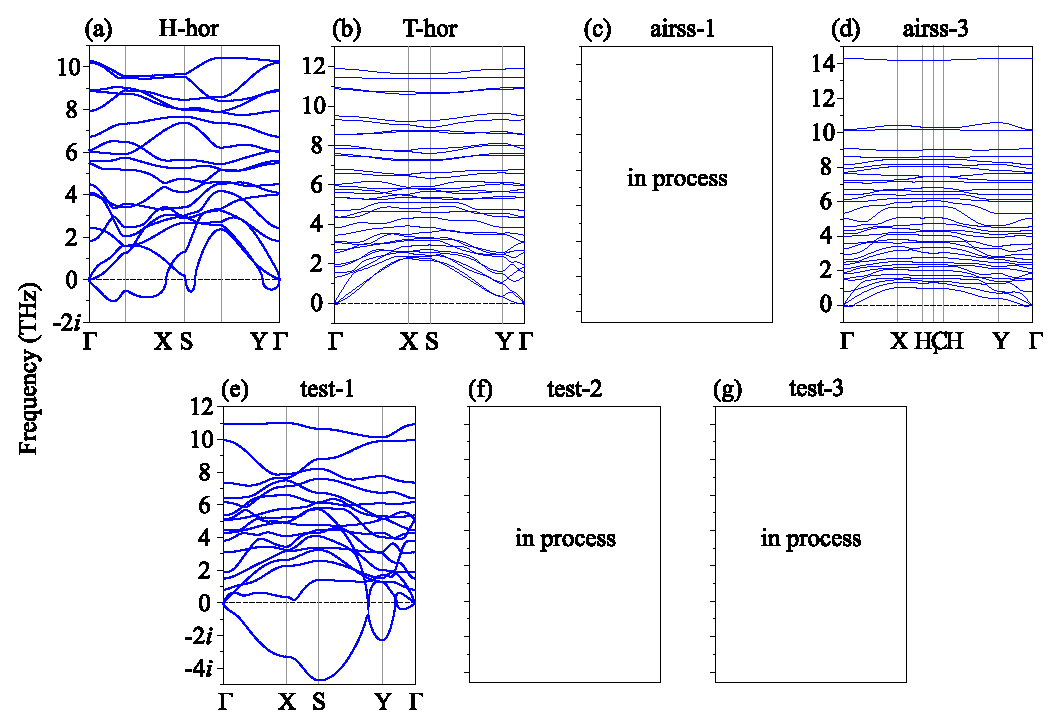
\includegraphics[width=\textwidth]{phon_svse.eps}
	\caption{Phonon dispersion curves of SVSe structures.}
	\label{phon_svse}
\end{figure}


\begin{figure}[H]
	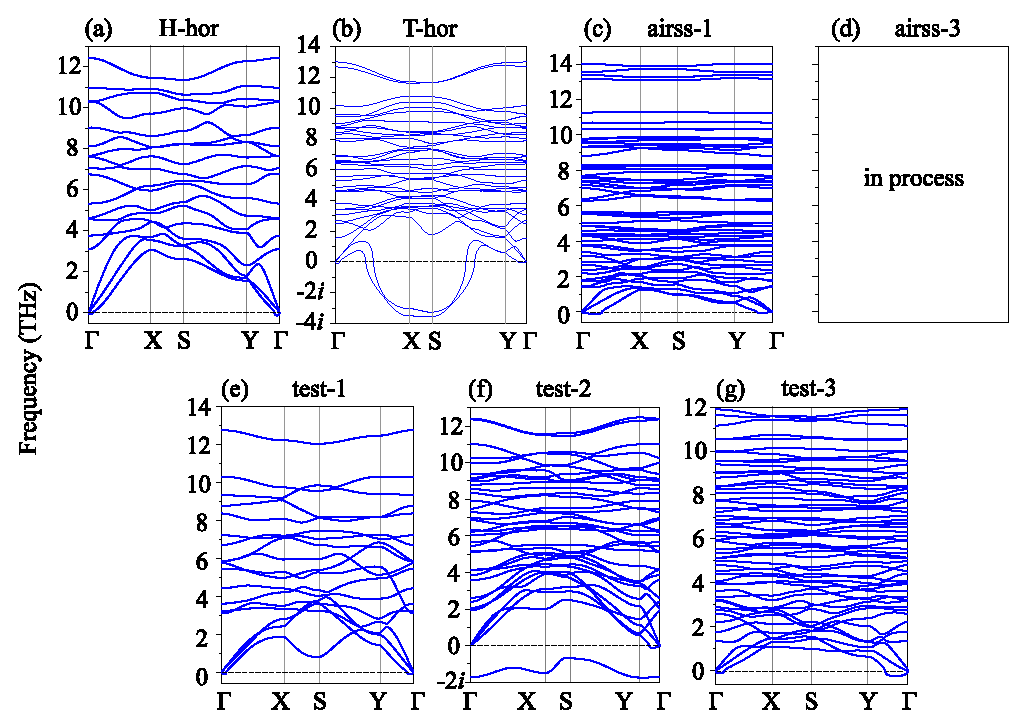
\includegraphics[width=\textwidth]{phon_smose.eps}
	\caption{Phonon dispersion curves of SMoSe structures. }
	\label{phon_smose}
\end{figure}


	\begin{longtable}[c]{l*{9}{l}}
	\caption{Predicted structures of SMoSe and SVSe} \label{t:str}  \\
		\hline
		\multirow{2}*{Phase}	& 	\multirow{2}*{Space group}	& \multicolumn{3}{c}{\multirow{2}*{Lattice parameters (\AA, deg)}}	&	\multirow{2}*{Atom}	&	\multicolumn{3}{c}{Coordinates} \\ 
		\cline{7-9}
		&&&&&&  x	&	y	&	z \\ 
		\hline
		SVSe & $Pm\ (\#6)$  &	$a=3.6955$ & $b=12.0193$ & $c=17.1112$  & V	&	0.0921	&	0.3413	&	0.4568	\\
		T-hor&&$\alpha$ = 90.000& $\beta$=90.605& $\gamma$ = 90.000& V	&	0.5882	&	0.8456	&	0.5342	\\
		1M&&&&&	S	&	0.6057	&	0.7696	&	0.4077	\\
		&&&&&	S	&	0.0633	&	0		&	0.5125	\\
		&&&&&	S	&	0.3174	&	0.5		&	0.3765	\\
		&&&&&	Se	&	0.1058	&	0.2737	&	0.5943	\\
		&&&&&	Se	&	0.5950	&	0.5		&	0.4940	\\
		&&&&&	Se	&	0.8148	&	0		&	0.6313	\\
		\hline 
		SMoSe & $Pm\ (\#6)$  &	$a=6.2189$ & $b=3.2228$ & $c=16.7225$  & Mo	&	0.5174	&	0	&	0.5164	\\
		H-hor&   &$\alpha$ = 90.000& $\beta$=98.670& $\gamma$ = 90.000 & Mo	&	-0.0928	&	0.5	&	0.4739	\\
		1M'&&&&&   S	&	0.1525	&	0	&	0.4276	\\
		&&&&& 	S 	&	0.6730	&	0	&	0.3962	\\
		&&&&&	Se	&	0.7587	&	0.5	&	0.6054	\\
		&&&&& 	Se	&	0.2676	&	0.5	&	0.5806	\\
		\hline
		SVSe & $P1\ (\#1)$  &	$a=6.6377$ & $b=10.2914$ & $c=26.7249$  & V  &	0.1701	&	0.0669	&	0.3384	\\	
		airss-1&&$\alpha$ = 89.797& $\beta$=87.588& $\gamma$ = 89.999& V &	0.2037	&	0.5653	&	0.2917	\\
		1A &&&&&	V	&	0.6964	&	0.0669	&	0.3384	\\
		&&&&&	V	&	0.6783	&	0.5653	&	0.2917	\\
		&&&&&	V	&	0.4392	&	0.8197	&	0.3025	\\
		&&&&&	V	&	-0.0652	&	0.3195	&	0.3282	\\
		&&&&&	S	&	0.4307	&	0.6327	&	0.3525	\\
		&&&&&	S	&	0.6642	&	0.2633	&	0.3753	\\
		&&&&&	S	&	0.1896	&	0.2633	&	0.3753	\\
		&&&&&	S	&	-0.0696	&	0.5416	&	0.3542	\\
		&&&&&	S	&	0.4263	&	-0.0539	&	0.3789	\\
		&&&&&	S	&	-0.0738	&	-0.0519	&	0.3793	\\
		&&&&&	Se	&	-0.0553	&	0.1313	&	0.2699	\\
		&&&&&	Se	&	0.7136	&	0.7671	&	0.2475	\\
		&&&&&	Se	&	0.1834	&	0.7671	&	0.2475	\\
		&&&&&	Se	&	0.4450	&	0.0514	&	0.2682	\\
		&&&&&	Se	&	-0.0507	&	0.4381	&	0.2430	\\
		&&&&&	Se	&	0.4493	&	0.4438	&	0.2426	\\
		\hline 
		SMoSe & $P1\ (\#1)$  &	$a=6.5969$ & $b=9.9921$ & $c=27.6937$  & Mo  &0.1478 &0.0694  &0.3275 \\
		airss-1&&$\alpha$ = 90.024& $\beta$=87.689& $\gamma$ = 89.999& Mo &0.641 &0.116 &0.165\\
		1A'&&&&&	Mo	&	0.7221	&	0.0694	&	0.3275	\\
		&&&&&	Mo	&	0.6522	&	0.5690	&	0.3013	\\
		&&&&&	Mo	&	0.4381	&	0.8084	&	0.3090	\\
		&&&&&	Mo	&	0.9362	&	0.3069	&	0.3201	\\
		&&&&&	S	&	0.4283	&	0.6344	&	0.3668	\\
		&&&&&	S	&	0.6622	&	0.2613	&	0.3706	\\
		&&&&&	S	&	0.1931	&	0.2613	&	0.3706	\\
		&&&&&	S	&	0.9297	&	0.5373	&	0.3583	\\
		&&&&&	S	&	0.4270	&	0.9651	&	0.3745	\\
		&&&&&	S	&	0.9269	&	0.9415	&	0.3749	\\
		&&&&&	Se	&	0.9470	&	0.1309	&	0.2562	\\
		&&&&&	Se	&	0.7177	&	0.7655	&	0.2526	\\
		&&&&&	Se	&	0.1776	&	0.7655	&	0.2526	\\
		&&&&&	Se	&	0.4456	&	0.0464	&	0.2644	\\
		&&&&&	Se	&	0.9485	&	0.4613	&	0.2478	\\
		&&&&&	Se	&	0.4483	&	0.4348	&	0.2488	\\
		\hline
		SVSe & $P1\ (\#1)$  &	$a=5.0351$ & $b=8.7721$ & $c=18.0178$  & V	&	0.2426	&	-0.0280	&	0.5623	\\
		airss-3&&$\alpha$ = 77.990& $\beta$=82.386& $\gamma$ = 78.789  & V	&	0.7676	&	0.0298	&	0.4302	\\		
		1A''&&&&&	V	&	0.1205	&	0.3274	&	0.4532	\\
		&&&&&	V	&	0.8752	&	0.6755	&	0.5417	\\
		&&&&&	S	&	0.2587	&	0.0491	&	0.4287	\\
		&&&&&	S	&	0.7713	&	0.7610	&	0.4083	\\
		&&&&&	S	&	0.6782	&	0.3075	&	0.4066	\\
		&&&&&	S	&	0.1493	&	0.6174	&	0.4231	\\
		&&&&&	Se	&	0.7462	&	-0.0417	&	0.5734	\\
		&&&&&	Se	&	0.2518	&	0.2363	&	0.5951	\\
		&&&&&	Se	&	0.3271	&	0.6790	&	0.5997	\\
		&&&&&	Se	&	0.8115	&	0.3867	&	0.5779	\\
		\hline
		SMoSe & $P1\ (\#1)$  &	$a=5.8488$ & $b=7.9475$ & $c=16.7618$  & Mo	&	0.3021	&	-0.0347	&	0.5433	\\
		airss-3&&$\alpha$ = 81.296& $\beta$ = 89.766& $\gamma$ = 80.752  & Mo	&	0.6998	&	0.0412	&	0.4549	\\		
		1A'''&&&&&	Mo	&	0.0300	&	0.3220	&	0.4832	\\
		&&&&&	Mo	&	-0.0365	&	0.6754	&	0.5074	\\
		&&&&&	S	&	0.3110	&	0.1015	&	0.4123	\\
		&&&&&	S	&	0.8422	&	0.8371	&	0.3825	\\
		&&&&&	S	&	0.7777	&	0.2944	&	0.3823	\\
		&&&&&	S	&	0.2581	&	0.5193	&	0.4402	\\
		&&&&&	Se	&	0.7063	&	-0.0971	&	0.5958	\\
		&&&&&	Se	&	0.1582	&	0.1749	&	0.6229	\\
		&&&&&	Se	&	0.2359	&	0.6904	&	0.6169	\\
		&&&&&	Se	&	0.7151	&	0.4759	&	0.5584	\\
		\hline
	\end{longtable}



%%%%%%%%%%%%%%%%%%%%%%%%
\subsubsection{Structures revealed with {\it unbiased} algorithms}
%%%%%%%%%%%%%%%%%%%%%%%
\paragraph{SVSe-1M structure}

The structure with monoclinic symmetry was predicted using USPEX for SVSe and was called SVSe-1M (T-hor). 
For SVSe composition it is more  energeticaly favourable than both 1H and 1T structure, although it is less favourable than 1T' (Figure \ref{t:enthalpy}).
Calculation of phonon dispersion curves have shown dynamic stability of SVSe-1M (Figure \ref{phon_svse}) and instability of SMoSe-1M (Figure \ref{phon_smose}) structures.


1M structure is characterized by the same octahedral coordination polyhedron as 1T structure.
The difference is in the arrangement of the coordination [TMSSe$_3$] octahedra.
As it was mentioned, in 1T structure octahedra share only common edges, while in 1M both edges and faces.
Both structures can be described within modular approach.
In this case, the module is the double row of octahedra connected through the common edges.
In Figure \ref{T_hor_T} one of such a double rows is the row consisting of the rows \# 2 and \# 3.
In 1M structure, the adjacent double layers are attached through the common faces  of the octahedra (the face I(II)III on the Figure \ref{T_hor_T}).
In 1T structure the interconnection is edge-sharing (the edge II'III' in Figure \ref{T_hor_T}). 
The interconnection of the adjacent double layers in 1M and 1T structure is illustrated in  Figure \ref{T_hor_slabs}.
The joining of the double layers through the common face is identical to the mirror reflection of the initial double layer in the plane going through this face.
Thus 1M structure can be obtained from 1T one by means of twinning operation.


The described rearrangement of coordination octahedra results in the sufficient rearrangement of V atoms, with the appearance of the zig-zag chains of V atoms connected by the shorter bonds (Figure \ref{T_hor_V}) and undulation of the whole structure (Figures \ref{T_hor_hcb}).
The nets of chalcogen atoms are not affected so much and in 1M structure it is topologically the same as that in 1T structure, although the difference of geometrical parameters is sufficient.
The angles between S--S bonds in SVSe-1M structure vary in the range 91.38-139.8\textdegree, while in SVSe-1T structure all the angles are equal to 120\textdegree (Figure \ref{T_hor_ch}).
The S--S bond lengths in 1M are in the range 3.45--3.87\AA, while in 1T all they are equal to 3.41 \AA (Figure \ref{T_hor_ch}).


\begin{figure}[H]
	\includegraphics[width=0.8\textwidth]{T_hor_T.png} \\
	\caption{Comparison of 1M and 1T crystal structures}
	\label{T_hor_T}
\end{figure}

\begin{figure}[H]
	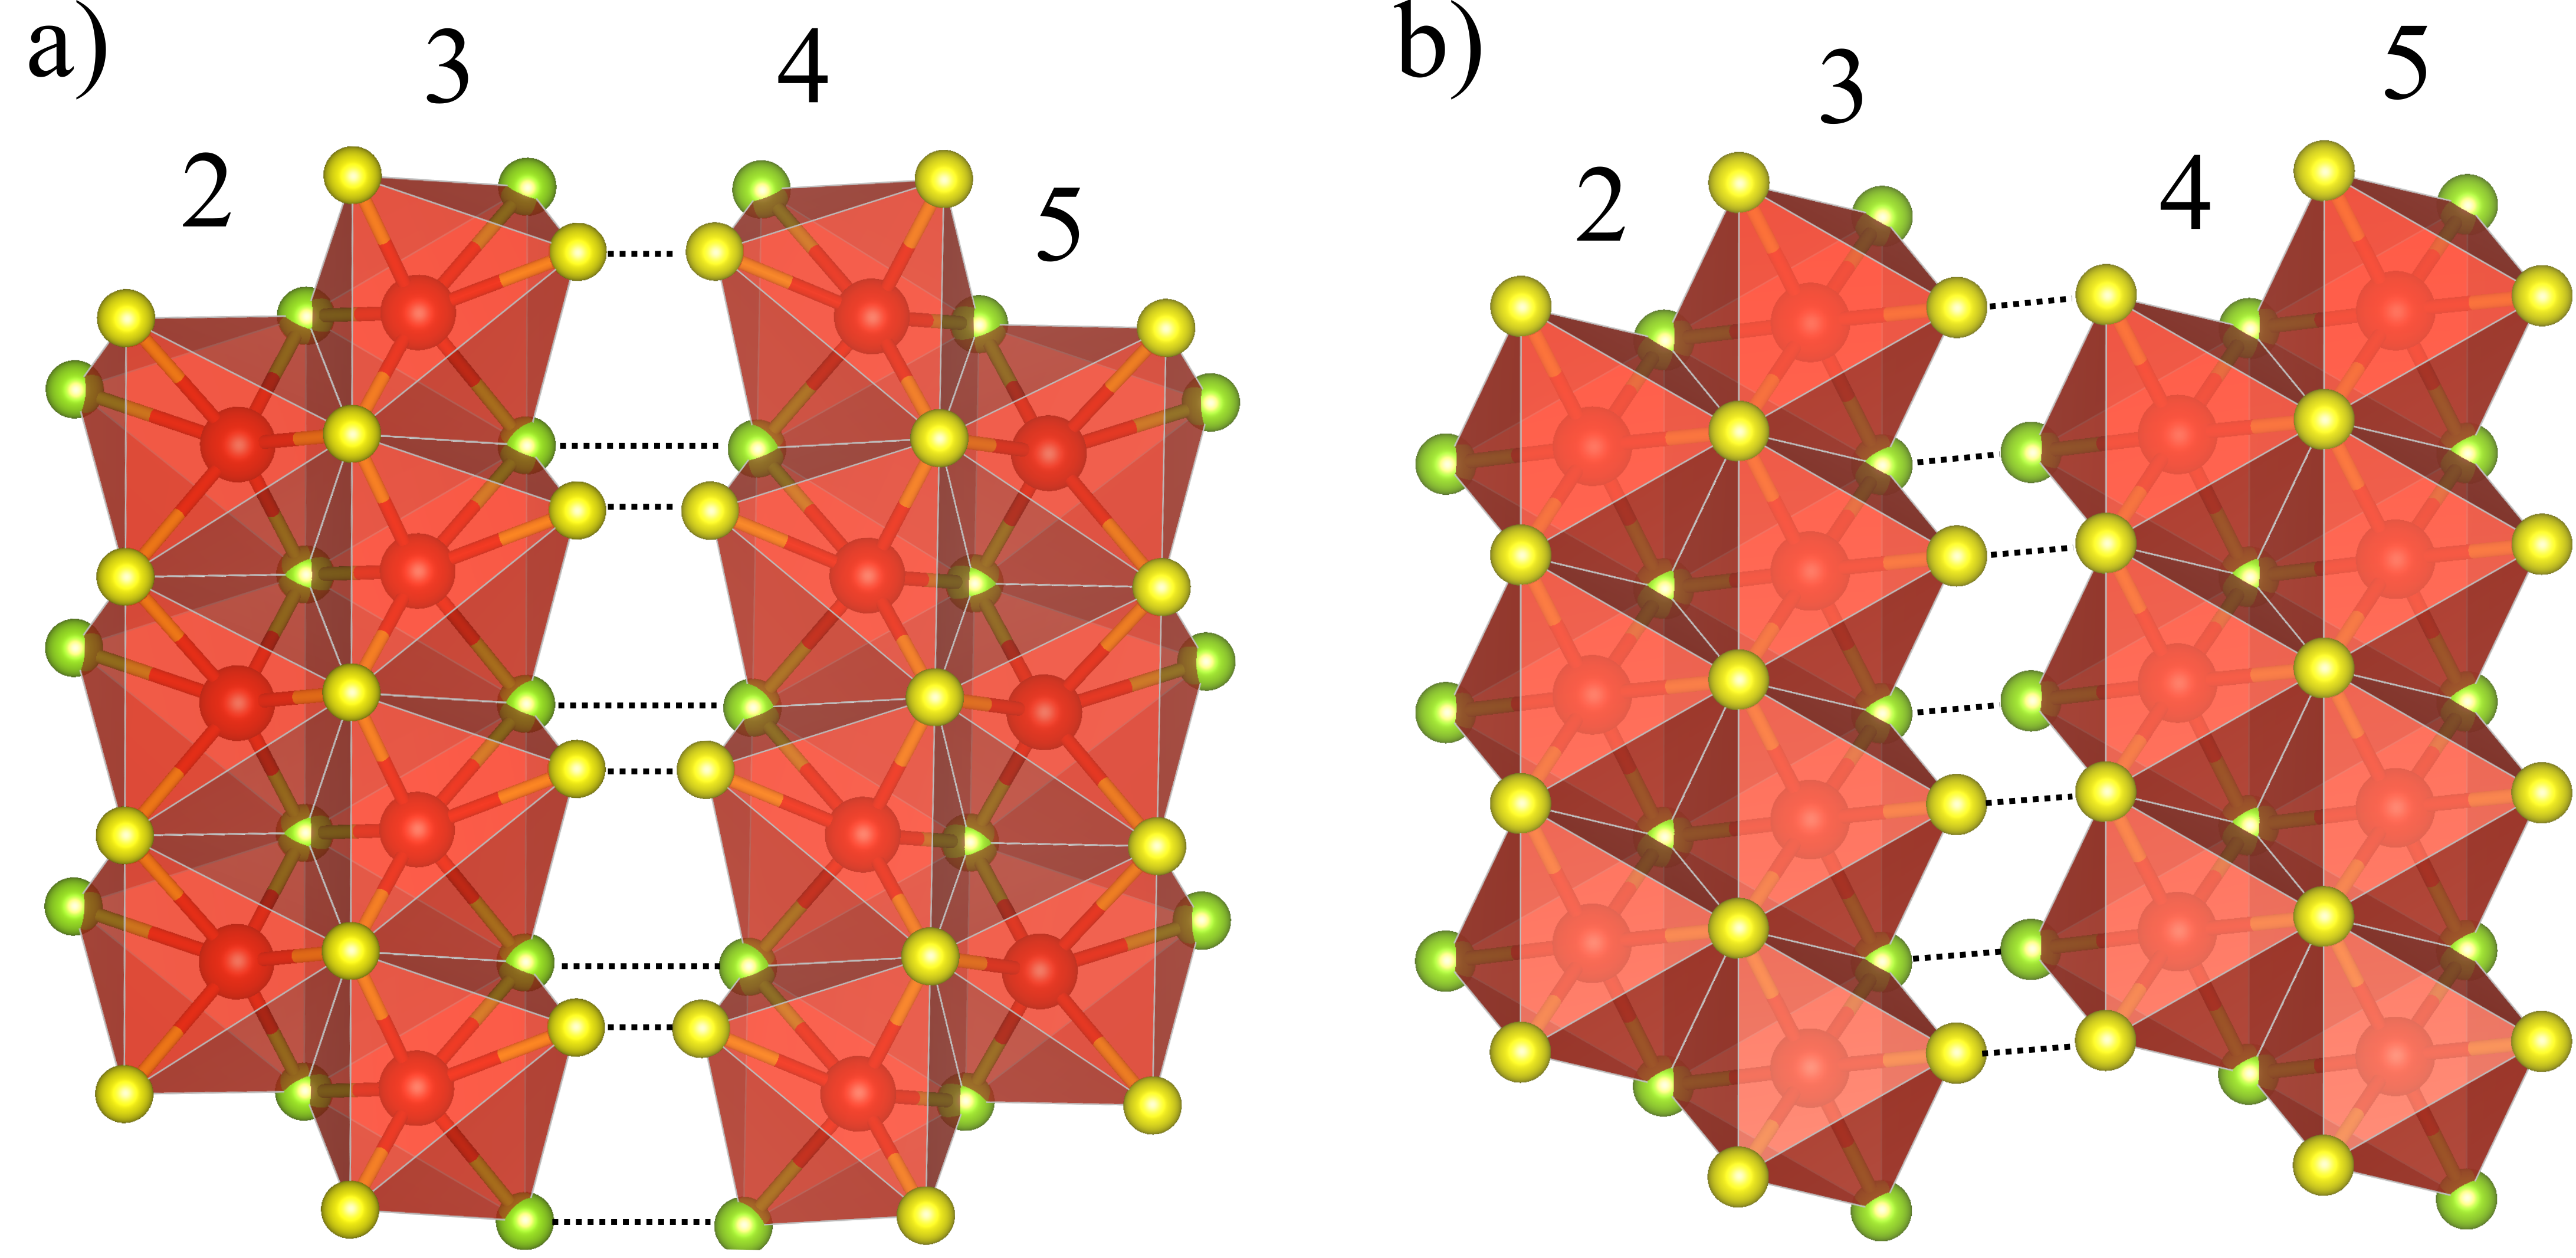
\includegraphics[width=0.7\textwidth]{T_hor_slabs.png} \\
	\caption{Arrangement of double octahedral rows in 1M (a) and 1T (b) structures; the dashed lines shows the common atoms in the adjacent slabs}
	\label{T_hor_slabs}
\end{figure}


\begin{figure}[H]
	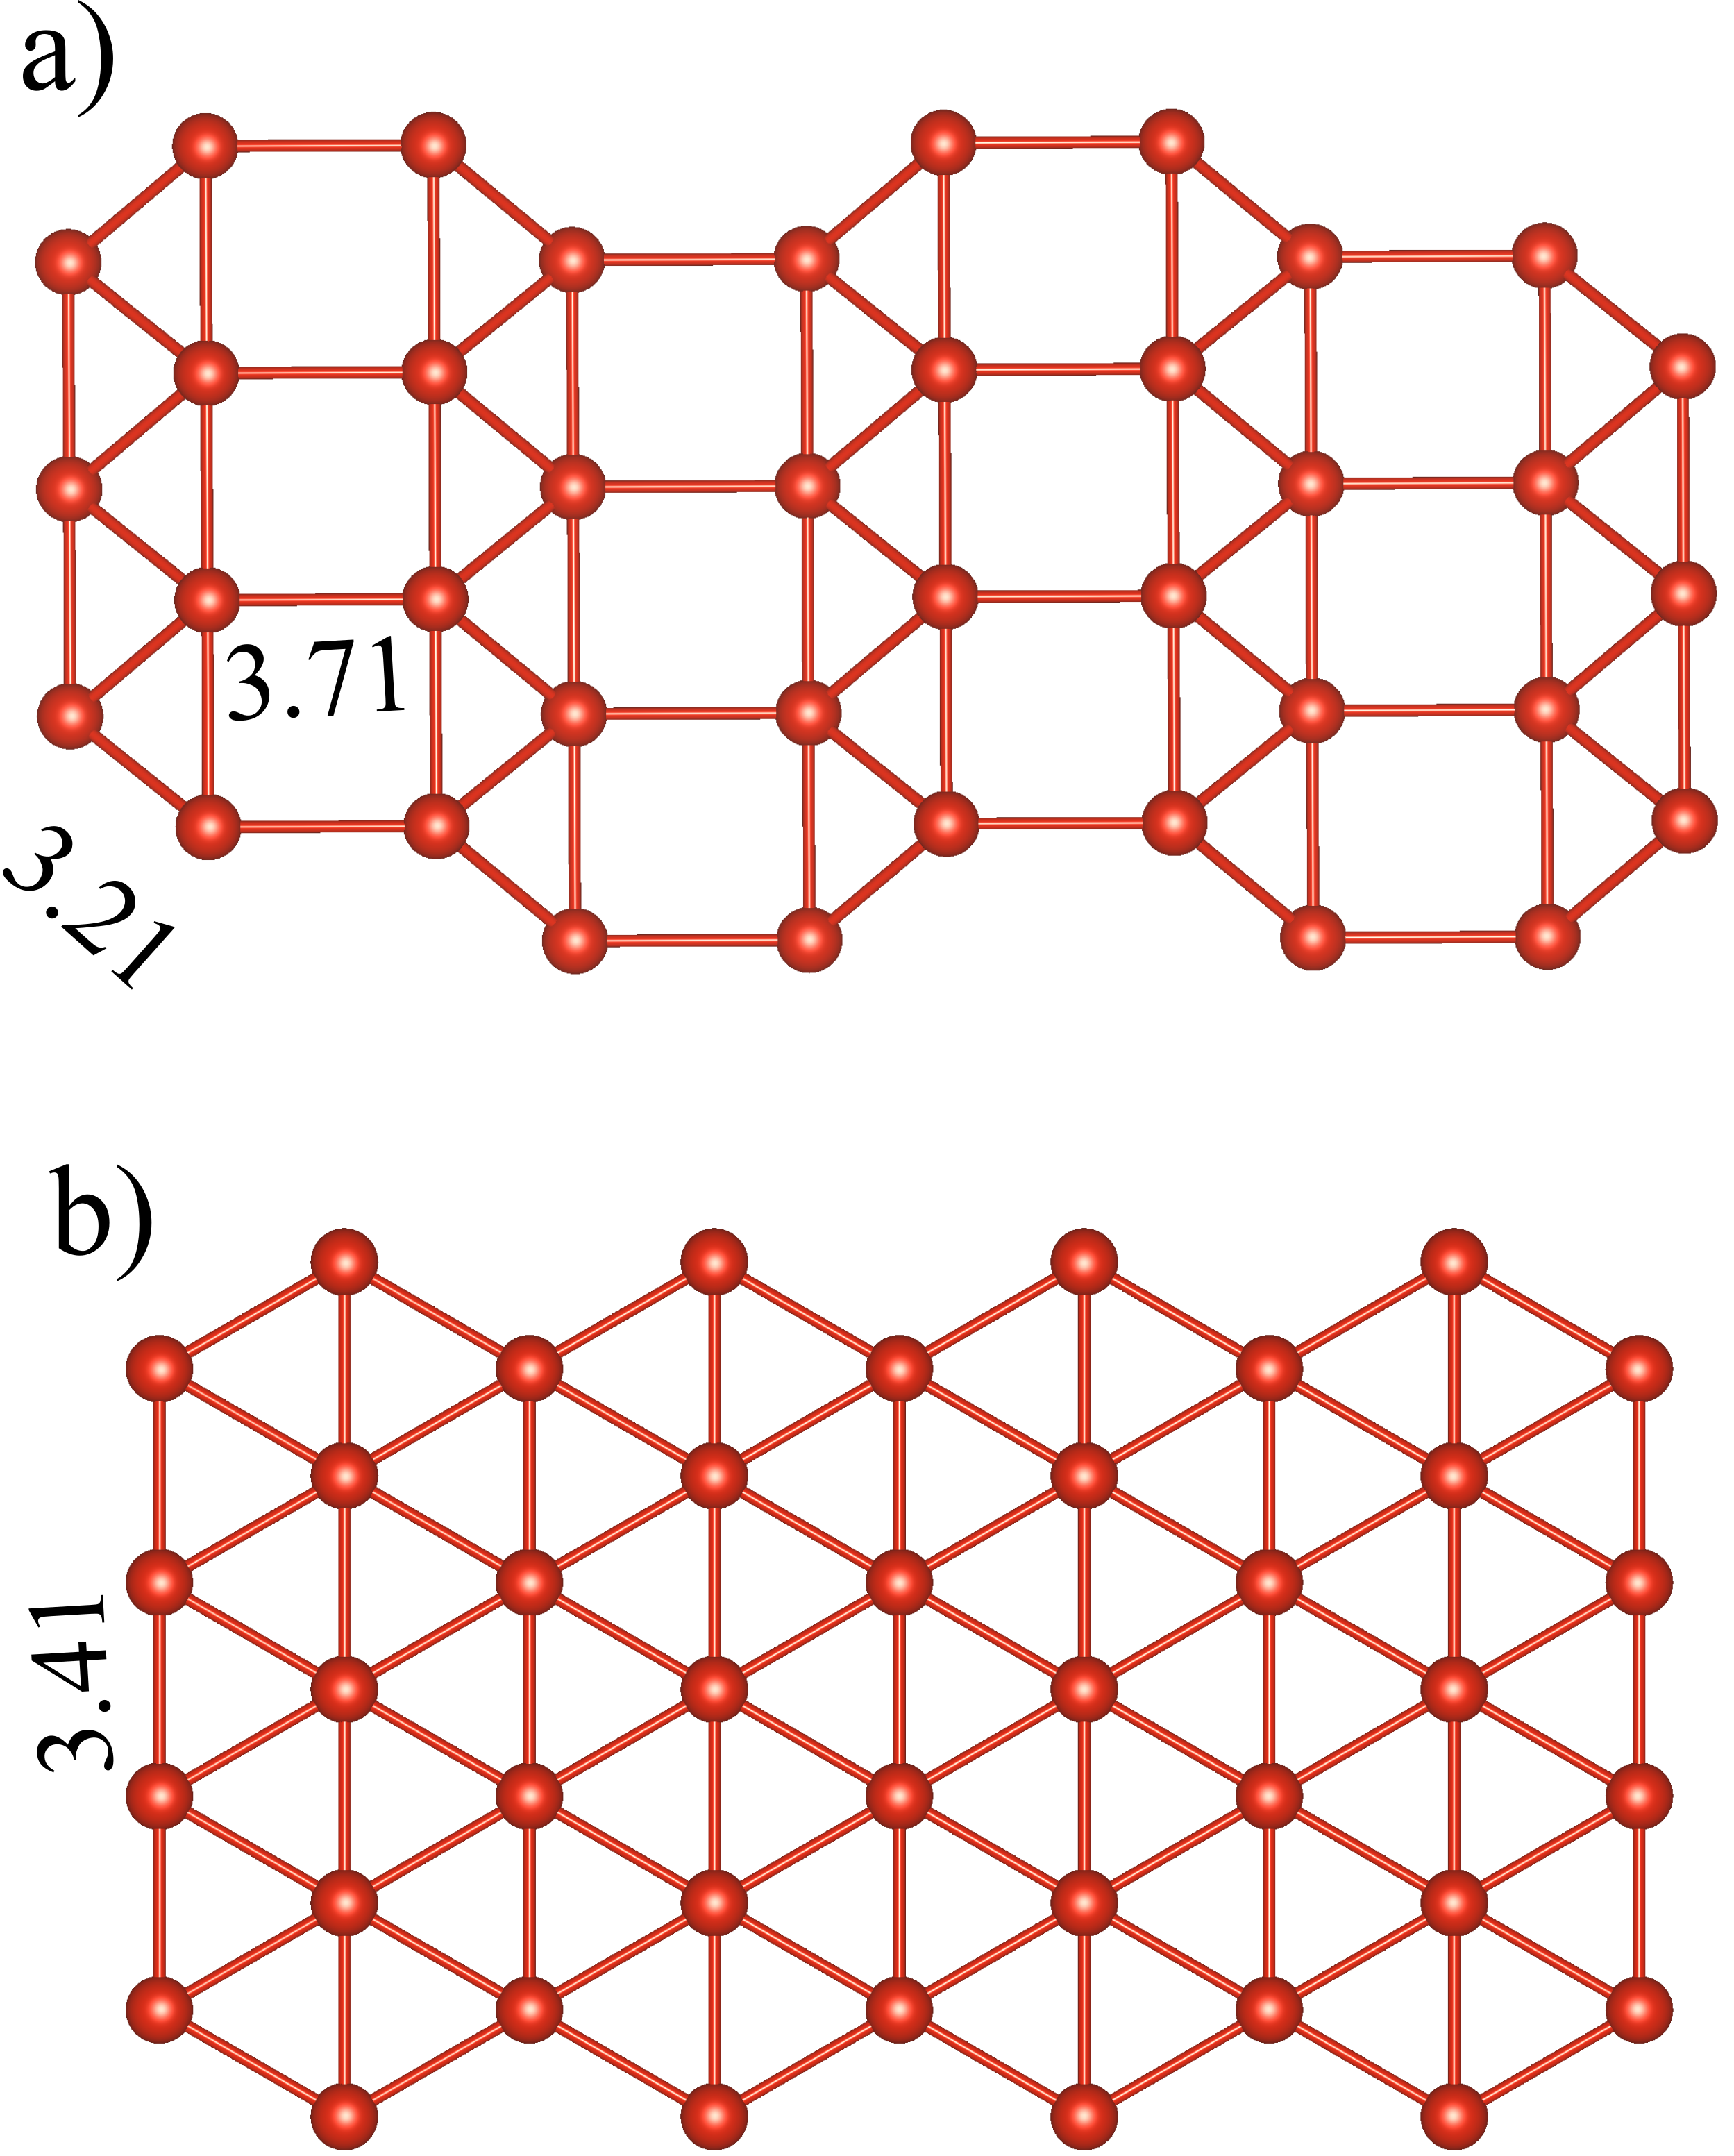
\includegraphics[width=0.4\textwidth]{T_hor_V.png} \\
	\caption{Comparison of the nets of TM atoms in 1M (a) and 1T crystal structures; values of interatomic distances are given in \AA.}
	\label{T_hor_V}
\end{figure}

\begin{figure}[H]
        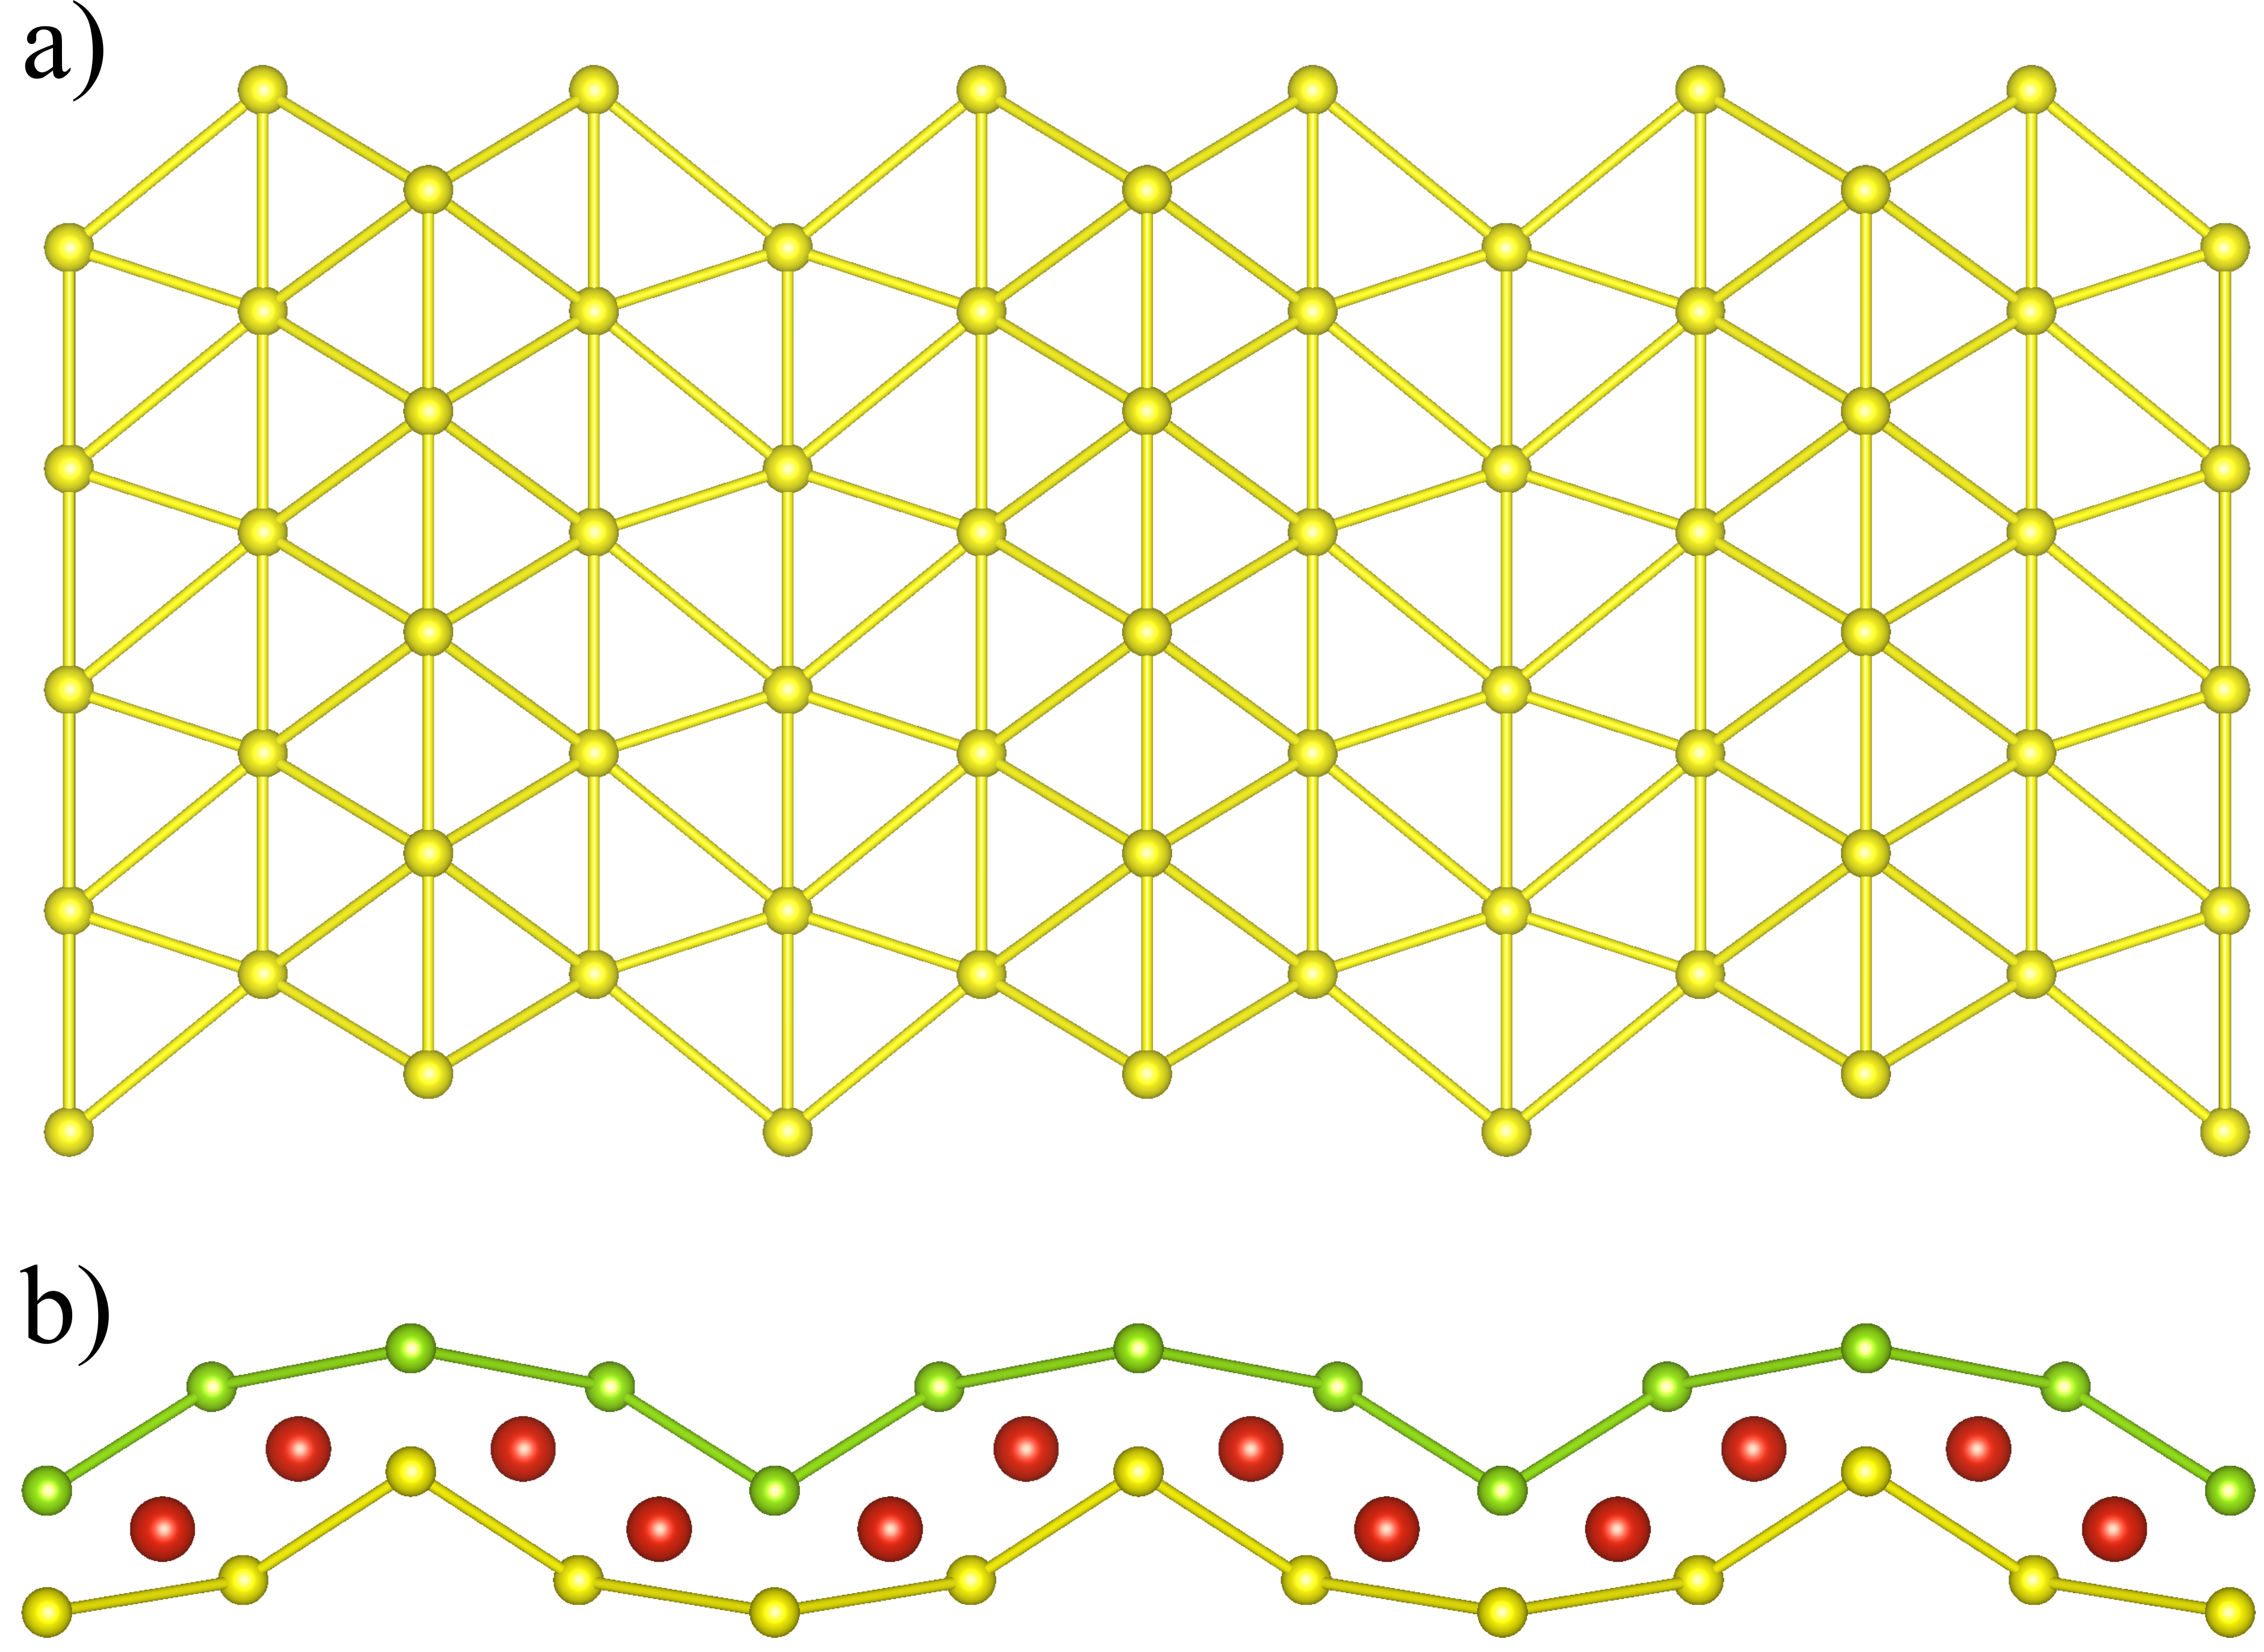
\includegraphics[width=0.5\textwidth]{T_hor_hcb.png} \\
        \caption{The undulated net of chalcogen atom in 1M structure: top- (a) and side-view (b)}
\label{T_hor_hcb}
\end{figure}


\begin{figure}[H]
	\includegraphics[width=0.5\textwidth]{T_hor_ch.png} \\
	\caption{Comparison of the nets of chalcogen atoms in 1M (a) and 1T crystal structures }
	\label{T_hor_ch}
\end{figure}


\paragraph{SMoSe-1M' (H-hor) structure}
Another structure with monoclinic symmetry sufficiently different from 1M structure was found using USPEX package for SMoSe composition.
This structure was named SMoSe-1M' (Table \ref{t:str}).
1M' structure is dynamically stable for SMoSe (Figure \ref{phon_smose}) composition and unstable for SVSe composition (Figure \ref{phon_svse}).


Enthalpy of SMoSe-1M' is higher than the enthalpy of 1T structure on 0.05 eV/f.u
It is as well higher than that of aforementioned 1M on 0.05 eV/f.u.

1M' structure is different from other structures in that it is characterized by the square net of chalcogen atoms.
The rings of the net are almost right squares (Figure \ref{H-hor}).
The bottom (selenium) layer is shifted relatively the top (sulfur) one (Figure \ref{H-hor}).
Transition metal atoms disposed in such a way to have trigonal prismatic coordination.
Similarly as it is in 1H, in 1M' structure trigonal prisms share only common edges, but not common faces.
Molybdenum atoms are connected by the bonds of 3.08--3.22 \AA\ lengths in quasi-1D chains.
The chains are connected by the sufficiently weaker bonds of 4.08 \AA\ length (Figure \ref{H-hor_Mo}).


\begin{figure}[H]
	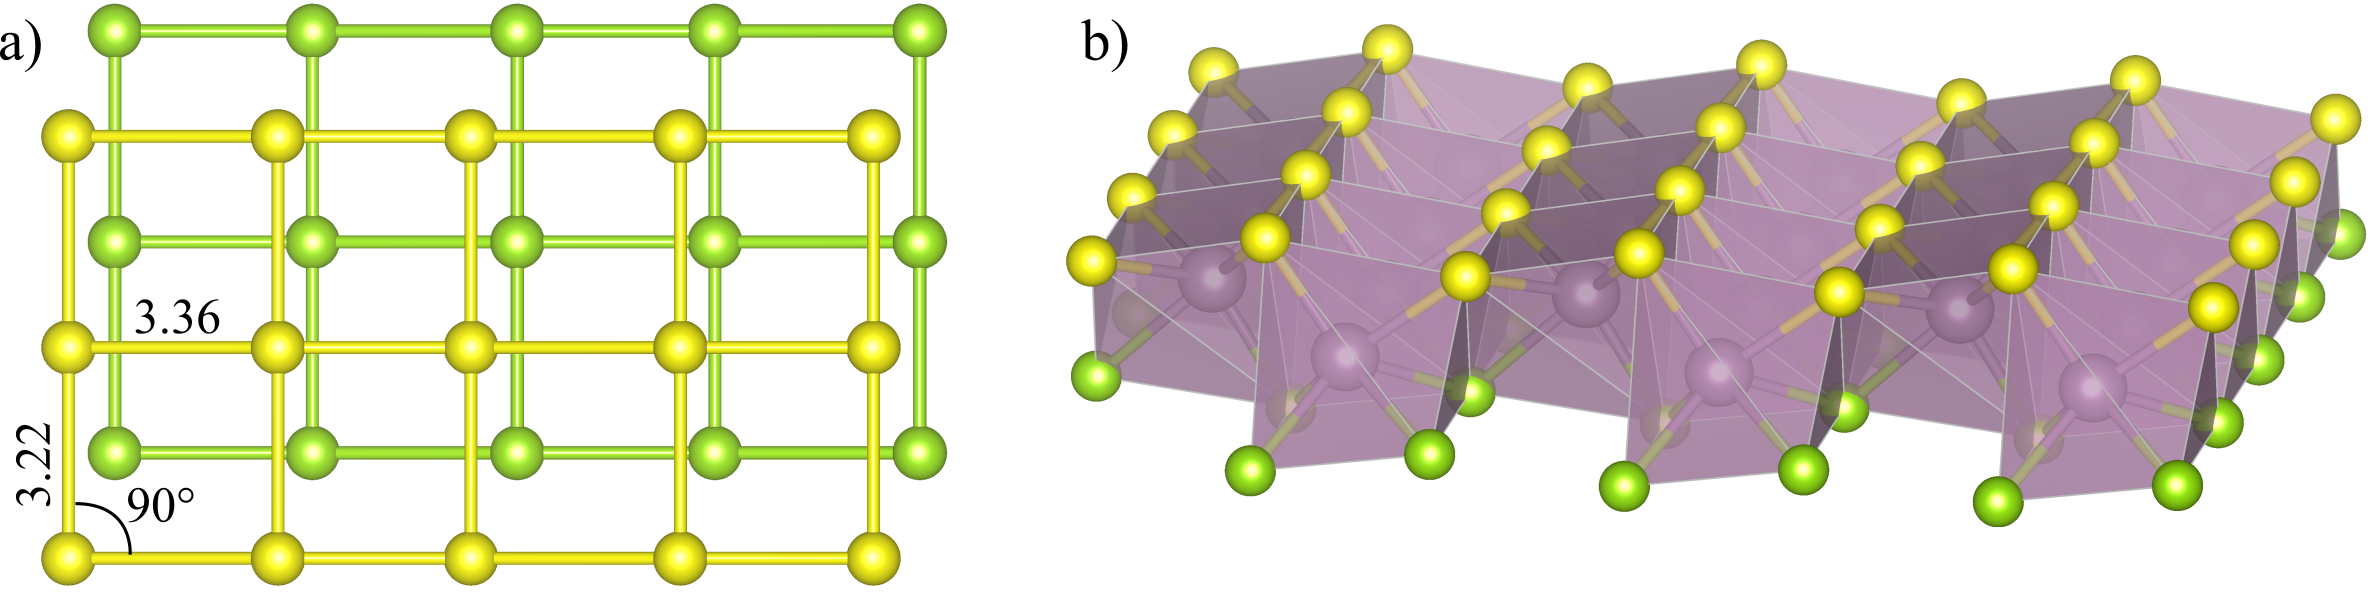
\includegraphics[width=\textwidth]{H-hor.png}
	\caption{Nets of sulfur (yellow) and selenium (green) atoms (a) and arrangement of coordination polyhedrons around Mo atoms (b) in SMoSe-1M' structure.}
	\label{H-hor}
\end{figure} 


\begin{figure}[H]
	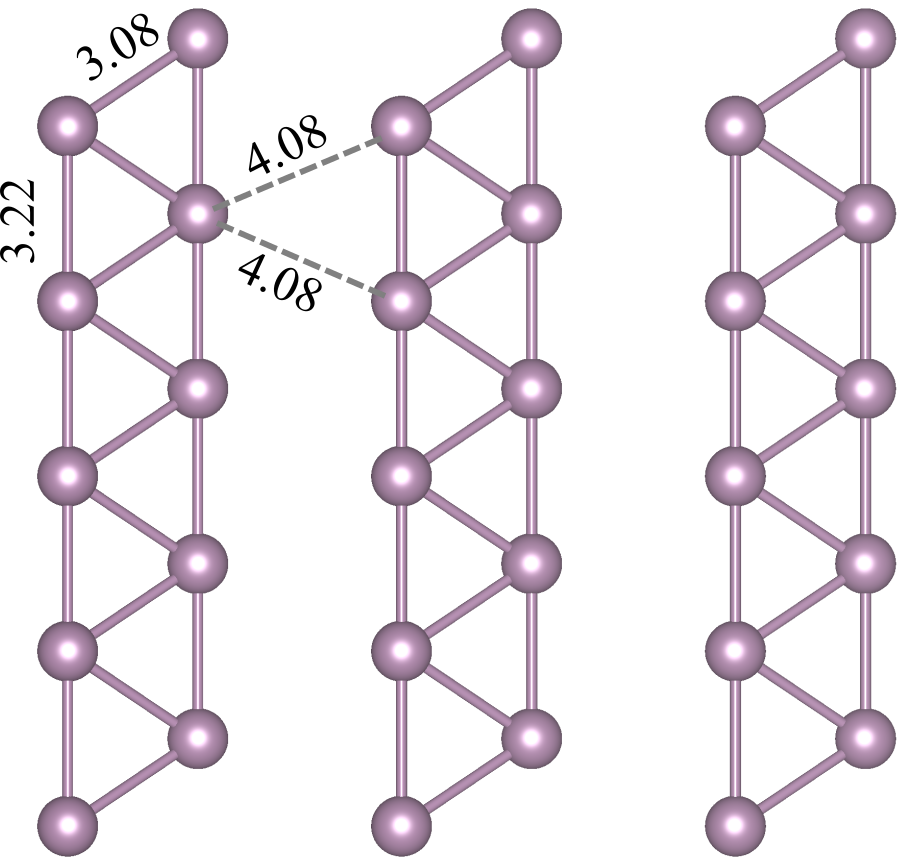
\includegraphics[width=0.4\textwidth]{H-hor_Mo.png}
	\caption{Chains of molybdenum atoms in SMoSe-1M' crystal structure.}
	\label{H-hor_Mo}
\end{figure} 


\paragraph{1A-SVSe and 1A'-SMoSe structures}
The structure with triclinic symmetry called 1A, was revealed with AIRSS package for SVSe compositions.
\textcolor{red}{(Тут наоборот, эта структура была предсказана для SMoSe, а потом мы ее примерили на SVSe)}
Despite sufficient structural similarity between optimized 1A structure for SMoSe and SVSe compositions there is apparent crystallographic difference between them, similar to that observed for 1T and 1T'.
Based on this we will designate them as 1A-SVSe and 1A'-SMoSe.
Both structures are dynamically stable (Figures \ref{phon_smose} and \ref{phon_svse}).

For 1A'-SMoSe, the enthalpy ratio is the following: $H(1T) > H(1A) > H(1T') > H(1H)$.
The enthalpy of 1A' structure in this case lies in-between values of enthalpies of 1T and 1T' structures, being more favourable than 1T on nearly 0.1 eV/f.u.
For 1A-SVSe -- $H(1T') < H(1T) < H(1H) < H(1A)$ and 1A' structure is less favourable than 1H on nearly 0.1 eV/f.u.


The structures 1A and 1A' can be better described based on the net of transition metal atoms, which forms the well known kagome lattice\cite{zhang2021_kagome}, observed for instance in AV$_3$Sb$_5$ \cite{ortiz2021} and WO$_3$ \cite{gerand1979} compounds.
In 1A'-SMoSe and 1A-SVSe, kagome lattices are not of ideal hexagonal symmetry, there is dispersion of bond lengths and deviation of bond angles from ideal values of 120\textdegree.
In 1A'-SVSe, the bond lengths vary in the range 3.07--3.49 \AA\ and bonds between the angles – in the rage 115-122.9\textdegree (Figure \ref{airss1_tm}).
In 1A'-SMoSe, the bond lengths are in the wide range of 2.78--3.79 \AA, and bond angles are in the range 113.9--125.7\textdegree.
1A'-SMoSe is different from 1A-SVSe in that it is characterized by the presence of triangular clusters of transition metal atoms with sufficiently shorter bond lengths.
The bond lengths within clusters are equal to 2.78--2.81 \AA, while other Mo--Mo bonds are on 0.5--1 \AA\ longer (Figure \ref{airss1_tm}).
In SMoSe-1T', the zig-zag chains of Mo atoms are connected by the bond of 2.79 \AA\ length, i.e. they are equal to the bond lengths within triangular clusters.
As it will be shown below, the formation of clusters and chains of molybdenum atoms are typical for the revealed structures.




The net of sulfur atoms in 1A and 1A' structures are different from that in 1T or 1H structures (Figure \ref{airss1_s}) but similar to each other (Figure \ref{airss1_s_comp}).
However sulfur net of 1A can be transformed into sulfur net of 1H (or 1T) by the shift, shown in the Figure \ref{airss1_s} and subsequent deformations.
Differences of bond angles and bonds lengths in 1A and 1A' structures do not exceed 0.1 \AA\ and 1\textdegree.
Net of sulfur atom is not planar, the aplanarity are nearly equal to $\pm$10\textdegree.

In 1A and 1A' structures, each transition metal atom is coordinated by  chalcogen atoms arranged in highly deformed tetragonal pyramids.
The composition of such pyramids are VS$_3$Se$_2$ or VS$_2$Se$_3$ (MoS$_3$Se$_2$ or MoS$_2$Se$_3$, respectively).
The bond distances between transition metal and chalcogen atoms varies in the range 2.26--2.58 \AA\ for 1A-SVSe and in the range 2.29--2.63 \AA\ for 1A'-SMoSe.
The pyramids are connected through the common edges of triangular groups of atoms, corresponding to the triangular rings of the mentioned kagome lattice (Figure \ref{airss1_poly}).
Between clusters there are the big holes -- the centers of hexagonals rings of kagome lattice \ref{airss1_poly}).



\begin{figure}
	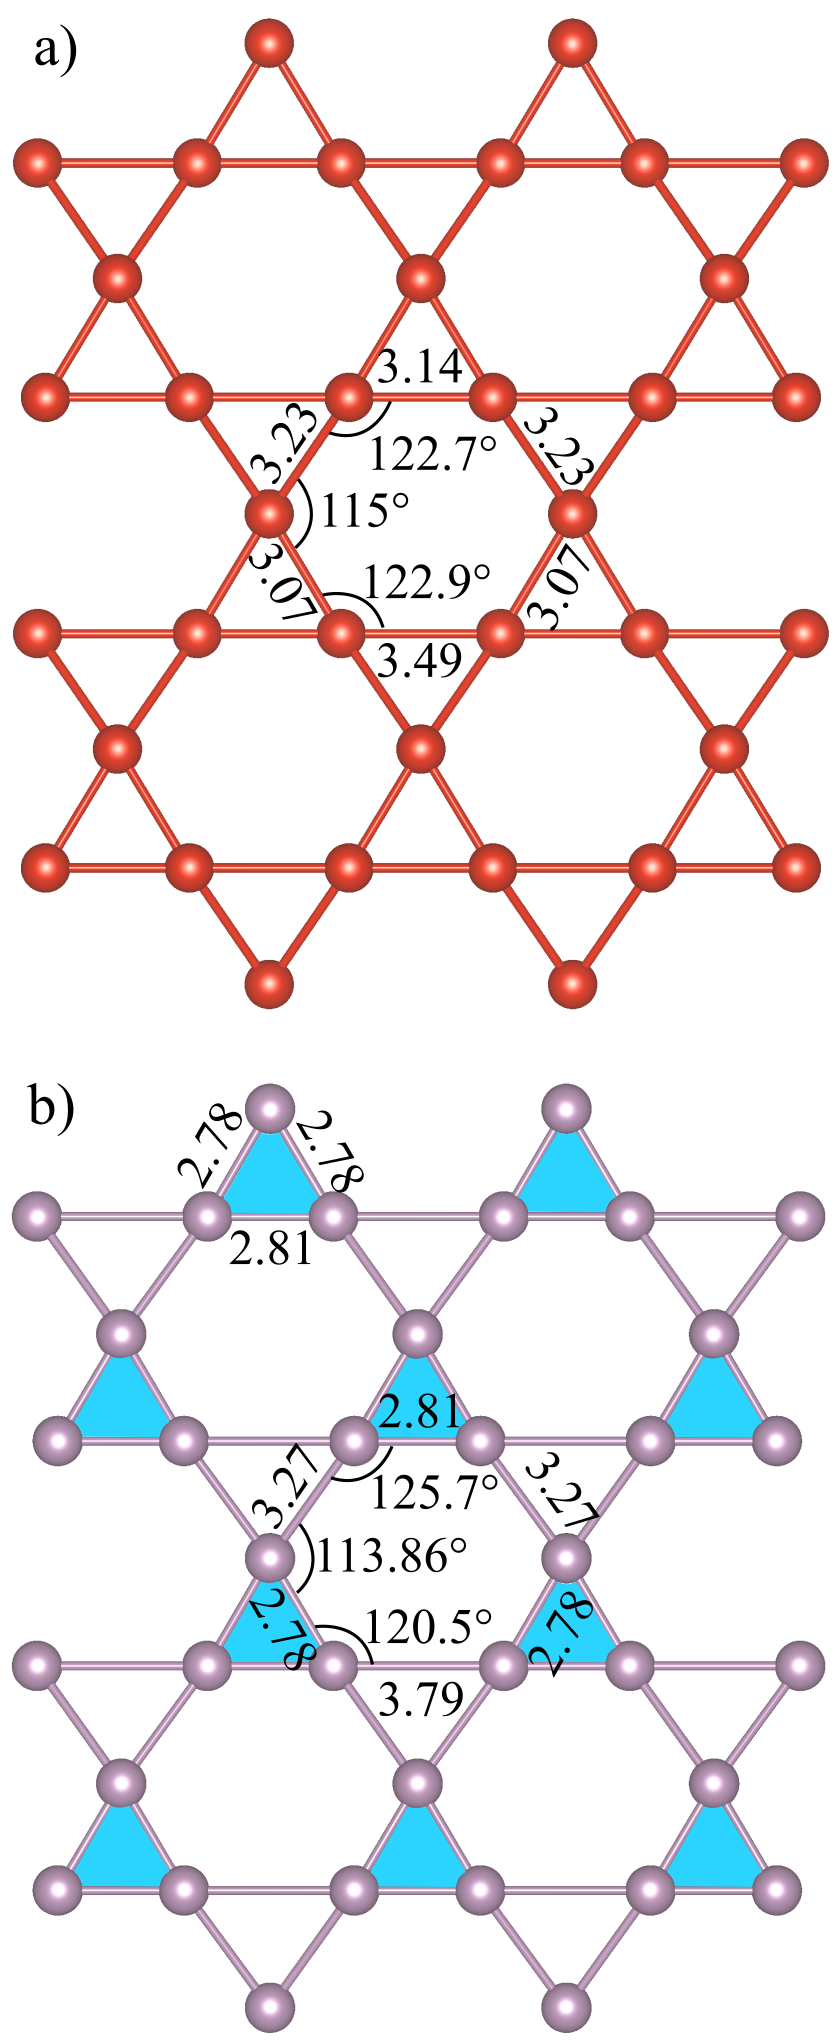
\includegraphics [width=0.35\textwidth]{airss1_tm.png}
	\caption{The kagome atomic nets of transition metal atoms in 1A'-SVSe (a) and SMoSe-1A (b); tringular clusters of Mo atoms are highlighted in blue} 
\label{airss1_tm}
\end{figure}

\begin{figure}
	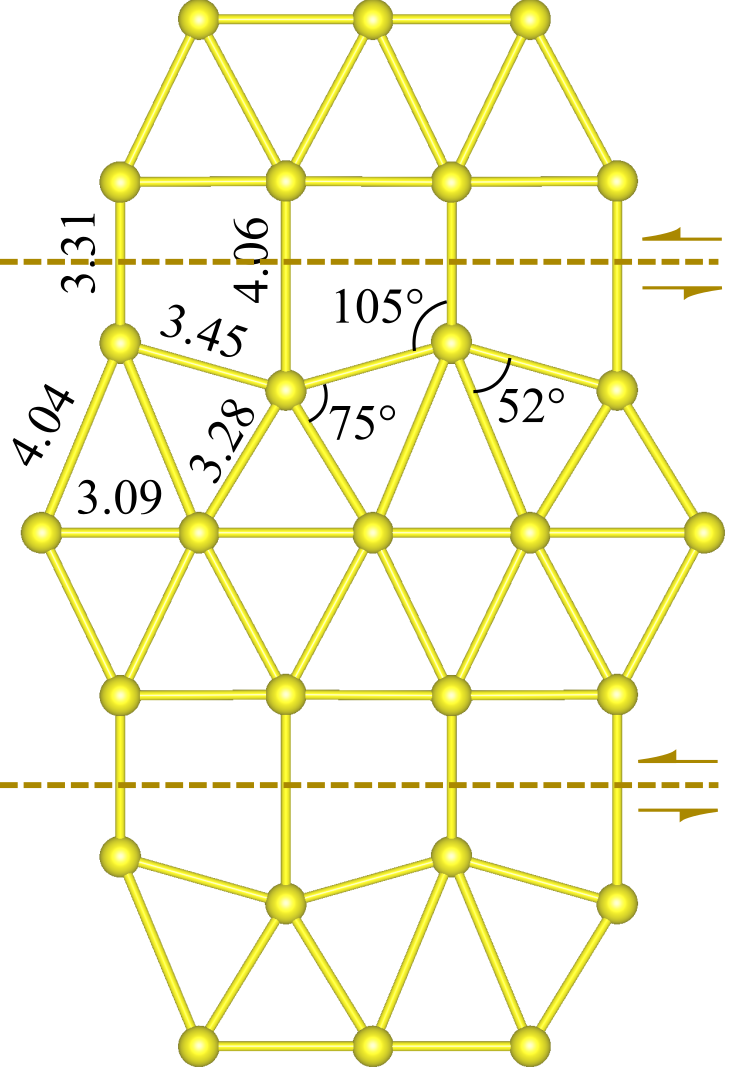
\includegraphics[width=0.35\textwidth]{airss1v_s.png}
	\caption{Net of sulfur atoms in 1A-SVSe; ; dashed line shows the plane of the shift transforming the net into the hexagonal net of 1T and 1H structures.}
\label{airss1_s}
\end{figure}


\begin{figure}[H]
        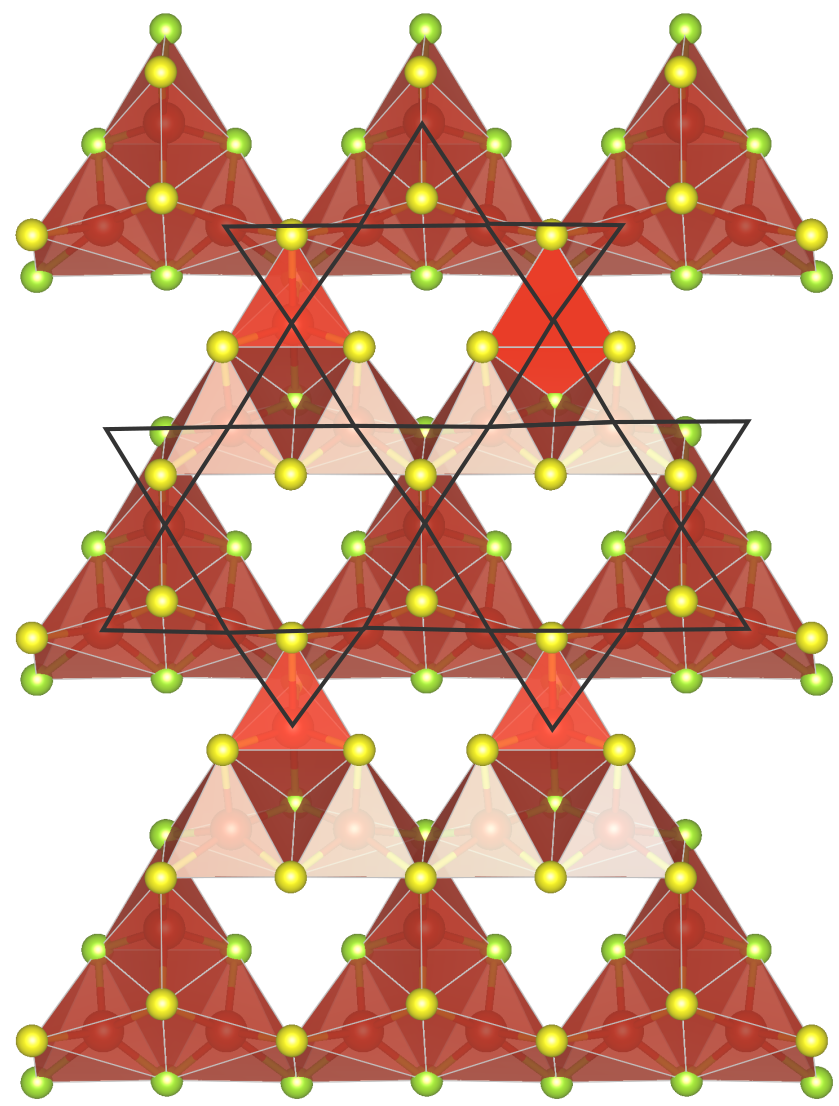
\includegraphics[width=0.35\textwidth]{airss1_v_poly.png}
        \caption{1A-SVSe with outlined coordination polyhedrons around V atoms; kagome lattice of V atoms is outlined in black.}
\label{airss1_poly}
\end{figure}




\paragraph{1A''-SVSe and 1A'''-SMoSe structures}
One more crystal structure with triclinic symmetry was revealed for SVSe composition with AIRSS code and them optimized for SMoSe compositions.
There are drastic difference between optimized SMoSe and SVSe structures and we will designate them as 1A''-SVSe and 1A'''-SMoSe.

Crystal structures  1A-SVSe and 1A'''-SMoSe give the good illustration for the different effects of vanadium and molybdenum atoms on the crystal structure of TMDs.
Both structures are dynamically stable.
1A''-SVSe is more favourable than 1S and 1H' structures on nearly 0.4 eV/f.u., while 1A'''-SMoSe is less favourable on the same value of energy.

Differences of 1A'' and 1A''' can be clearly seen in the side-view.
In 1A''-SVSe atoms of TM are nearly in the same plane as sulfur and selenium while in 1A'''-SMoSe structure they are between the layers of sulfur and selenium.

The nets of chalcogen atoms are also sufficiently different.
In 1A''-SVSe the topology of the net corresponds to the graphite-like hexagonal net, while in 1A'''-SMoSe chalcogen atoms form triangular net, if the weak contacts of 4.58-4.64 \AA\ are considered.
The new crystallchemical feature of 1A''-SVSe which was not observed for the other TMDs structures, is the presence of S--S and Se--Se dimers with the bond length of 2.09 \AA\ and 2.37 \AA\, respectively (Figures \ref{airss3_svse}a and \ref{airss3_S_Se}).
These bond lengths corresponds to the lengths of the bonds in the crystals structures of elemental sulfur and selenium.
Other S--S and Se--Se bonds of 1A''-SVSe in  sufficiently longer, varying in the range 3.17--3.73 \AA\ (Figures \ref{airss3_svse}a and \ref{airss3_S_Se}).
In 1A'''-SMoSe there ano nor clusters of chalcogen atoms and S--S bond lengths vary in the range 3.24-3.79 \AA\ with the weak contacts of 4.58--4.64 \AA\ length (Figure \ref{airss3_svse}a).

The nets of transition metals are also drastically different which can be seen from the figures \ref{airss3_svse}b and \ref{airss3_smose}b.
1A'''-SMoSe is characterized by the presence of Mo--Mo dimers with the bond lenghts of 2.85 \AA, while other bonds vary in the range 3.04--3.74 \AA\ (Figure \ref{airss3_smose}b).
There is no such a short bonds in 1A''-SVSe, in which V--V bonds smoothly vary in the range 3.32--3.79 \AA.

TM atoms in 1A''-SVSe are five and six-coordinated by chalcogen atoms (Figure \ref{airss3_poly}a).
Coordination polyhedra are  deformed tetragonal pyramid and trigonal prism, respectively.
In 1A'''-SMoSe, TMs are four- and five-coordinated, with coordination polyhedra of the deformed tetrahedron and trigonal bipyramid (Figure \ref{airss3_poly}b).
1A''-SVSe is characterized by the infinite quadruple chains of coordination polyhedra (Figure \ref{airss3_poly}a) and 1A'''-SMoSe -- by the signle chains (Figure \ref{airss3_poly}b).
Within the chains in 1A'' and 1A''' structures, coordination polyhedra are connected through the common edges (Figure \ref{airss3_poly}).
The adjacent chains in 1A''-SVSe are connected through the common edges, while in 1A'''-SMoSe -- through the common edges (Figure \ref{airss3_poly}).

\begin{figure}[H]
	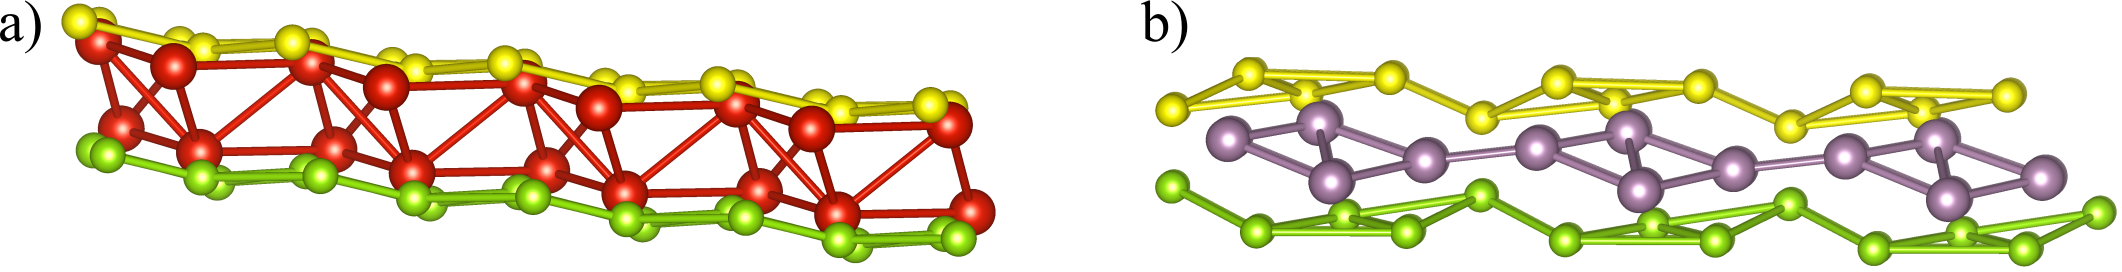
\includegraphics[width=\textwidth]{airss3_side.png}
	\caption{The side-view of 1A''-SVSe (a) and 1A'''-SMoSe (b) structures}
	\label{airss3_side}
\end{figure}

\begin{figure}[H]
	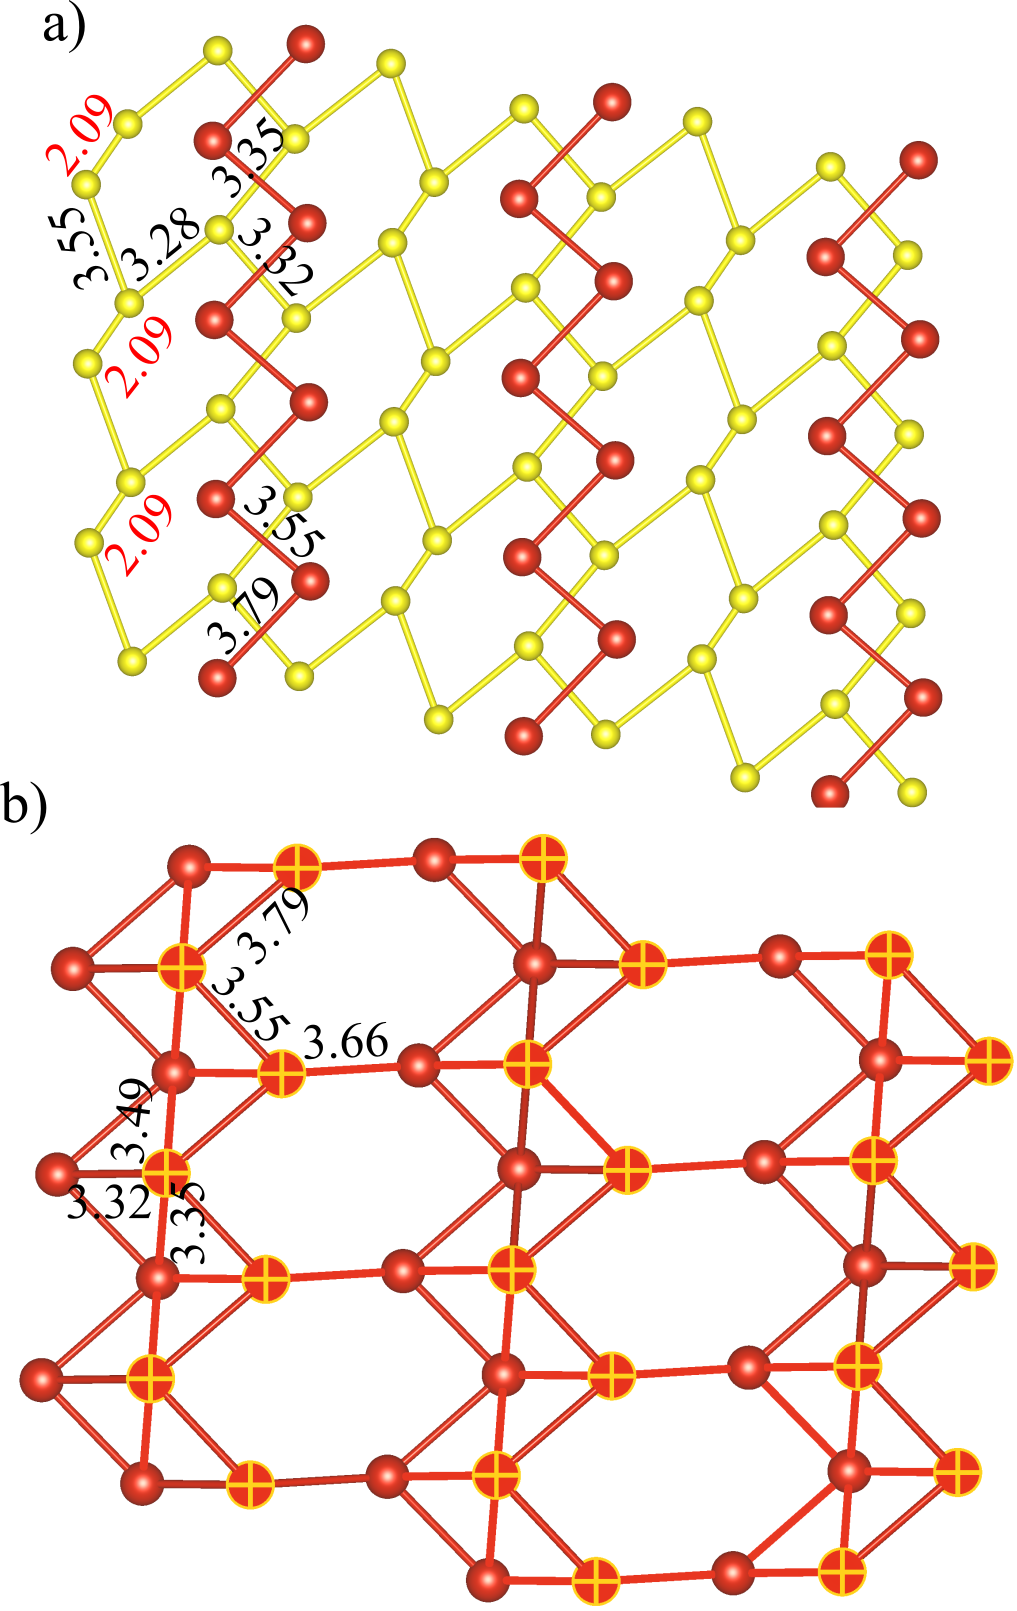
\includegraphics[width=0.5\textwidth]{airss3_svse.png}
	\caption{The net of sulfur (a) and vanadium (b) atoms in 1A''-SVSe}
	\label{airss3_svse}
\end{figure}

\begin{figure}[H]
	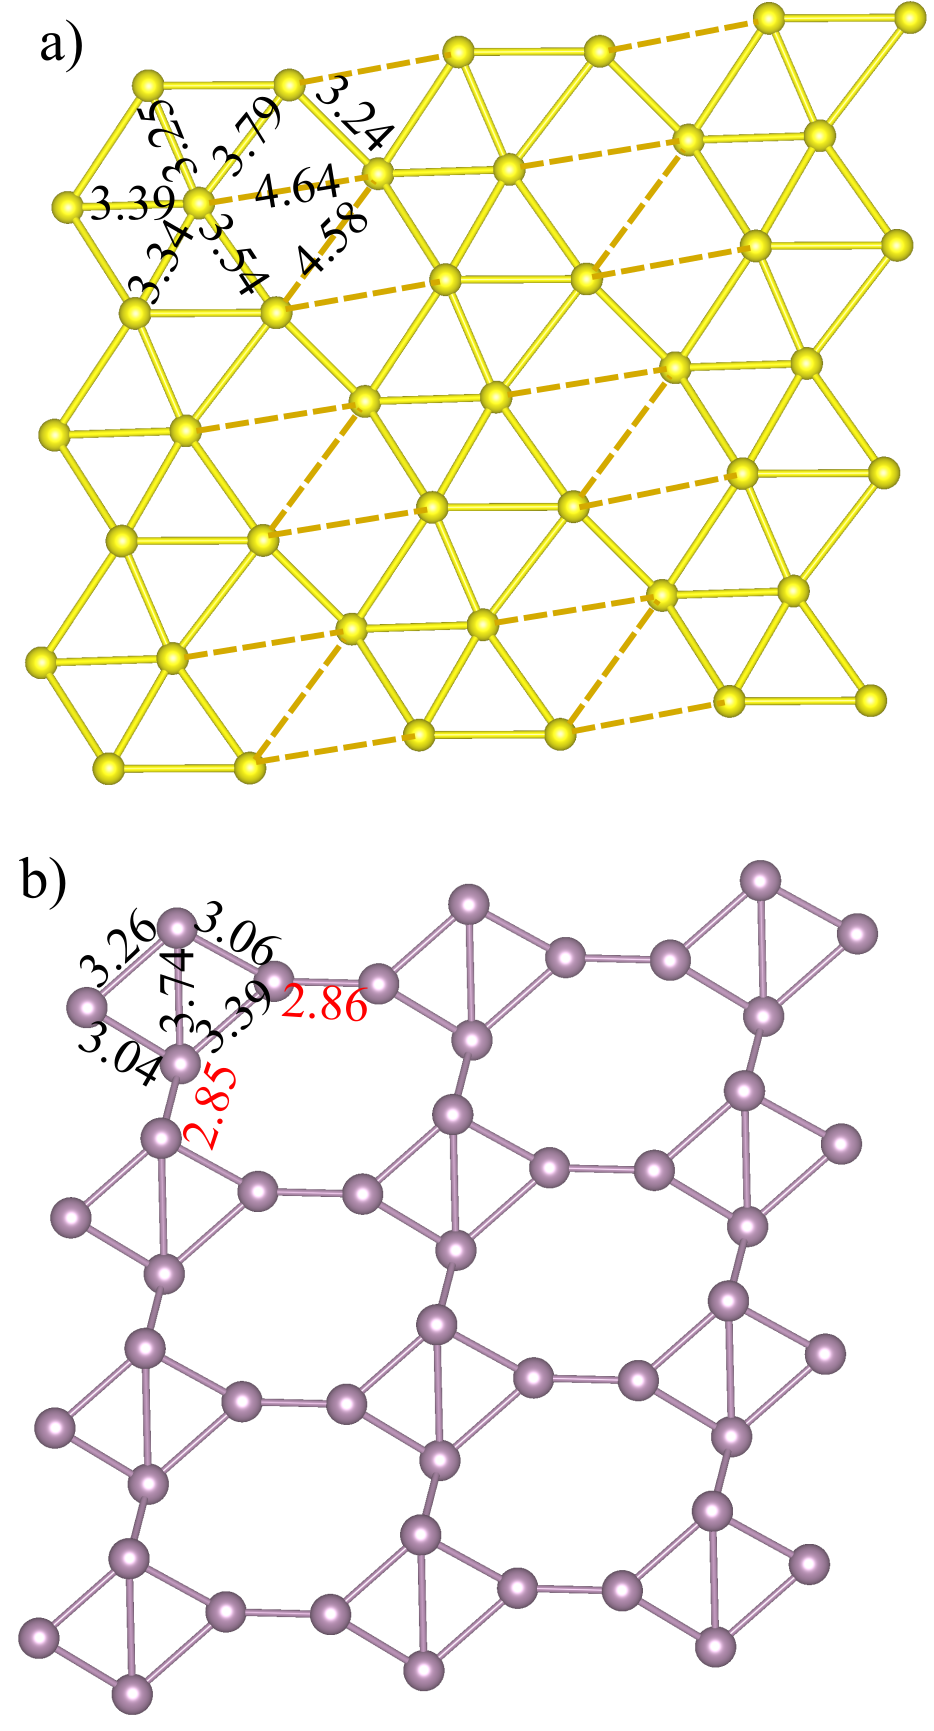
\includegraphics[width=0.5\textwidth]{airss3_smose.png}
	\caption{The net of sulfur (a) and molybdenum (b) atoms in 1A'''-SMoSe }
	\label{airss3_smose}
\end{figure}


\begin{figure}[H]
	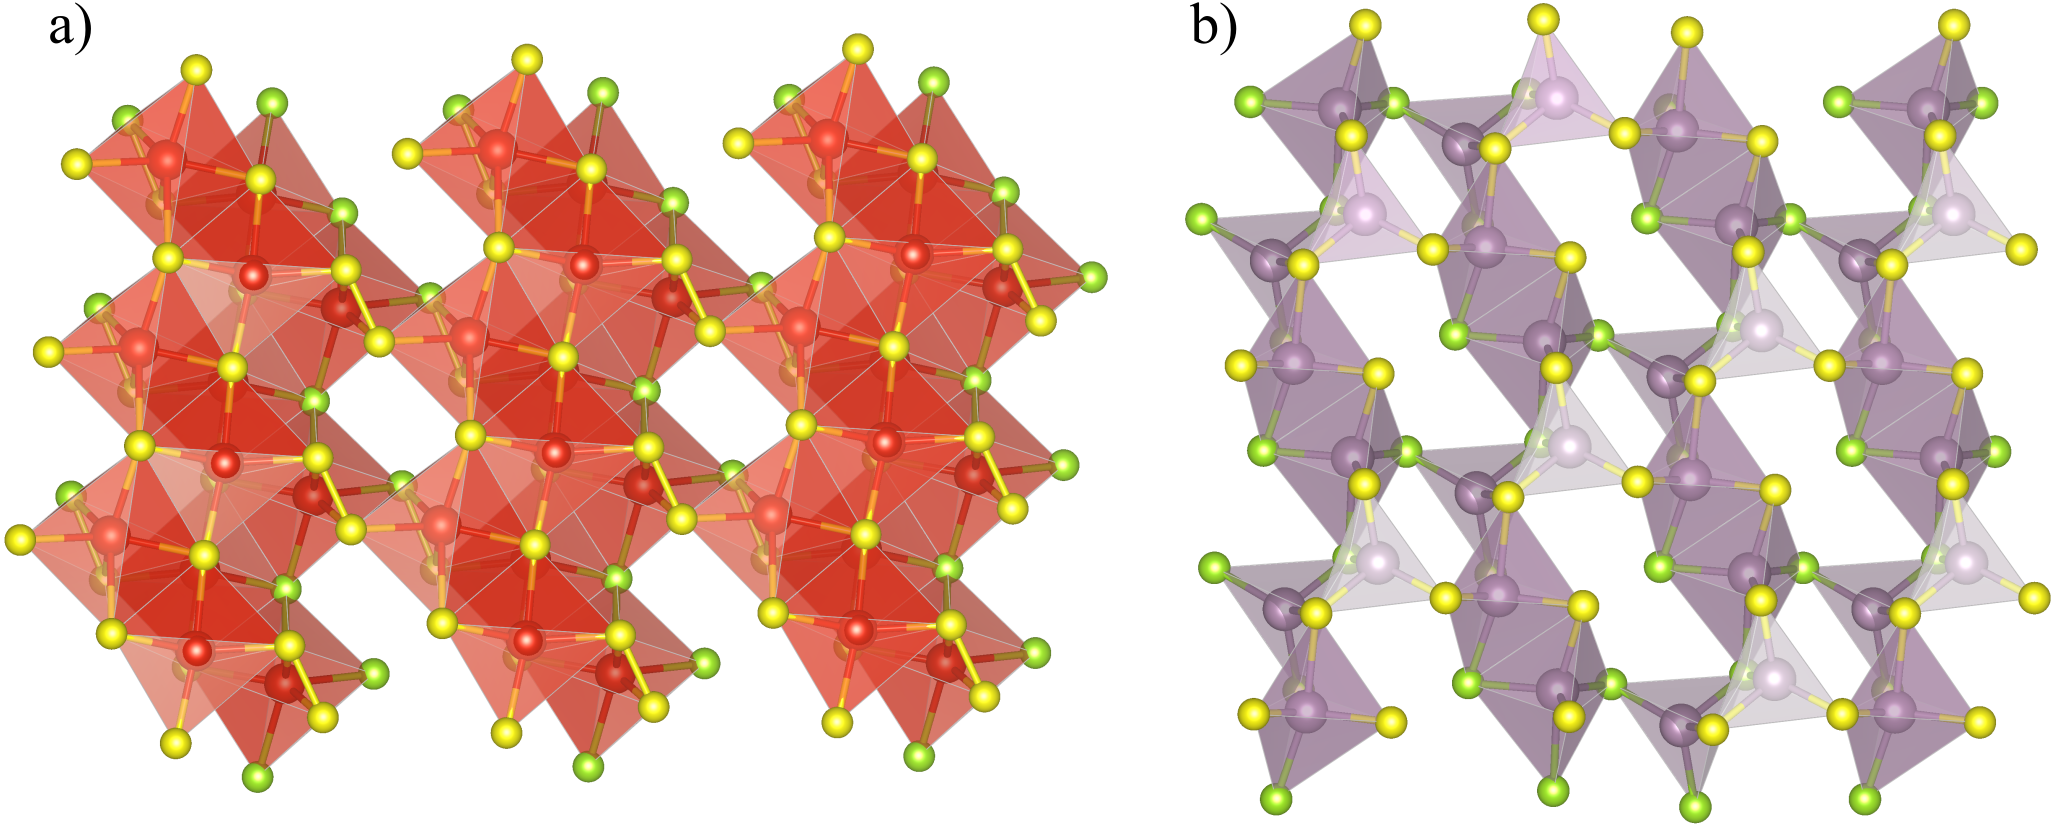
\includegraphics[width=\textwidth]{airss3_poly.png}
	\caption{Crystal structures 1A''-SVSe (a) and 1A'''-SMoSe (b) with outlined coordination polyhedra}
	\label{airss3_poly}
\end{figure}




%%%%%%%%%%%%%%%%%%%%%%%%%%%
\subsubsection{Structures produced manually based on 1H structure}
%%%%%%%%%%%%%%%%%%%%%%%%%%

In this section we consider crystal structures produced manually based on the 1H structure by the procedure which can be also used for the generation of the 1H' and 1S structures.
These structures, similarly to 1H' and 1S, can be considered as the possible structural models of grain boundaries.
As it will be shown below, enthalpies of the obtained strucrures are higher then the enthalpies of not only 1H, 1T and 1T' but also 1H' and 1S.
However, we add their desription hear together with the description of 1H' and 1S, to illustrate the formation of molybdenum dimers in SMoSe structures.
Also we would like to describe the procedure of structure generation, which can be also applied for the generation of the other similar structures.

To produce new structures with trigonal prismatic coordination of TM atoms, we present the structures as different fillings of the hexagonal nets of sulfur of 1H structure (Figure \ref{H-based}).
1H structure presents the most symmetric chess-board-like filling (Figure \ref{H-based}a).
The 1S structure can be also considered as the chess-board filling, but with the doubled triangular cells, having the form of rhombuses (Figure \ref{H-based}b).
After optimisation, these rhombuses transform into the right squares (Figure \ref{H-based}b).
In 1H' structure, the empty rings are of two types.
The first are primitive (non-centered) triangles, and the second are face-centered hexagons consisting of six triangular rings connected through the faces (Figure \ref{H-based}c).
The optimisation does not sufficiently change the forms of the empty rings, slightly deforming hexagons (Figure \ref{H-based}c).
In SMoSe and SVSe compositions, both 1H' and 1S are energetically less favourable than predicted H-hor, 1M and airss-1.
In one case, for H-hor and 1H' structures of SMoSe composition, enthalpies can be considered as equal within the error of the method.

Three new structures were produced in the similar way as it has been done for 1H' and 1S.
Two structures have the orthorhombic symmetry and one – the monoclinic one.
We will designate them O (test1), O' (test2), and M'' (1M''), respectively.
Structural data of SMoe-O, O', and M'' are given in {\it Supporting information} (Table \ref{t:str_test})
These structures are not dynamically stable for SVSe composition (Figure \ref{phon_svse}), and for SMoSe composition 1O and 1M'' are stable, while 1O' are not (Figure \ref{phon_smose}).
For SMoSe composition enthalpis of dynamically stable 1O and and 1M'' structures are higher than that of  1S and 1H' on nearly 0.1 eV/fu.

We failed to produce new structures obeying the local charge balance, i.e. the structures in which each vertex of the trigonal prism is common for three prisms, as it is in 1H, 1H' and 1S.
In the structure 1O, sulfur atoms are common for two or four trigonal prisms, in 1O' and 1M'' – for two or three, or four trigonal prisms (Figure \ref{H-based}).
1M'' structure is different from the other structures in that it is characterized by the presence of trigonal prisms with two common faces, while in all other structures prisms has no more than one common face.
As it will be shown below, this is important for the formation of Mo--Mo dimers.
Optimisation of 1M'' structure sufficiently affects the arrangement of sulfur atoms.
In the optimized 1M'' structure, the net of sulfur atoms is not more the hexagonal one (Figure \ref{H-based}f).
Mo atoms are not only in trigonal prismatic but also in quadratic coordination (Figure \ref{H-based}f).


Presence of common edges and faces of [MoO$_6$] trigonal prisms in 1H', 1S, 1O, 1O', and 1M'' structures results in shorter Mo--Mo distances in comparison with 1H structure, where prisms have only common edges.
In 1H structure, Mo atoms form regular hexagonal net with all Mo--Mo bonds being equal to 3.25 \AA.
This bond length corresponds to the edge sharing disposition of trigonal prisms.
In 1H', 1S, and 1O structures Mo--Mo distances for edge sharing disposition in prisms are equal to 2.9--3.8 \AA.
For face sharing disposition, the Mo--Mo distances is sufficiently shorter.
In 1H' and 1S tructers they are equal to 2.9 \AA, in 1O -- to 2.75 \AA and in 1O' -- to 2.62 \AA.
These distances are close to the Mo--Mo distances in the zig-zag chains of Mo atoms in 1T' structure (2.75 \AA).
This value is in turn equal to the shortest distance between Mo atoms in the {\it bcc} structure of pure Mo (2.72 \AA) \cite{MoV}.
1M'' structure is characterized by the sufficiently shorter Mo--Mo bond.
The distance between the adjacent Mo atoms in dimer is equal to 2.22 \AA.
This short bond corresponds to the quadruple Mo--Mo bond in Mo$_2^{4+}$ dimers, found in numerous organic molecules \cite{momo}.
Similarly to orgnic molecules, in 1M'' structure  each molybdenum atom of Mo--Mo dimer bound to four ligand atoms that define almost right square (Figure \ref{test3_momo}).
Despite the relatively high enthalpy of 1M'' structure, its dynamic stability show theoretical possibility for the formation of quadruply bonded Mo$_2^{4+}$ dimers in metastable structures of TMDs.
The possibility which was not considered before.

\begin{figure}[H] \centering
        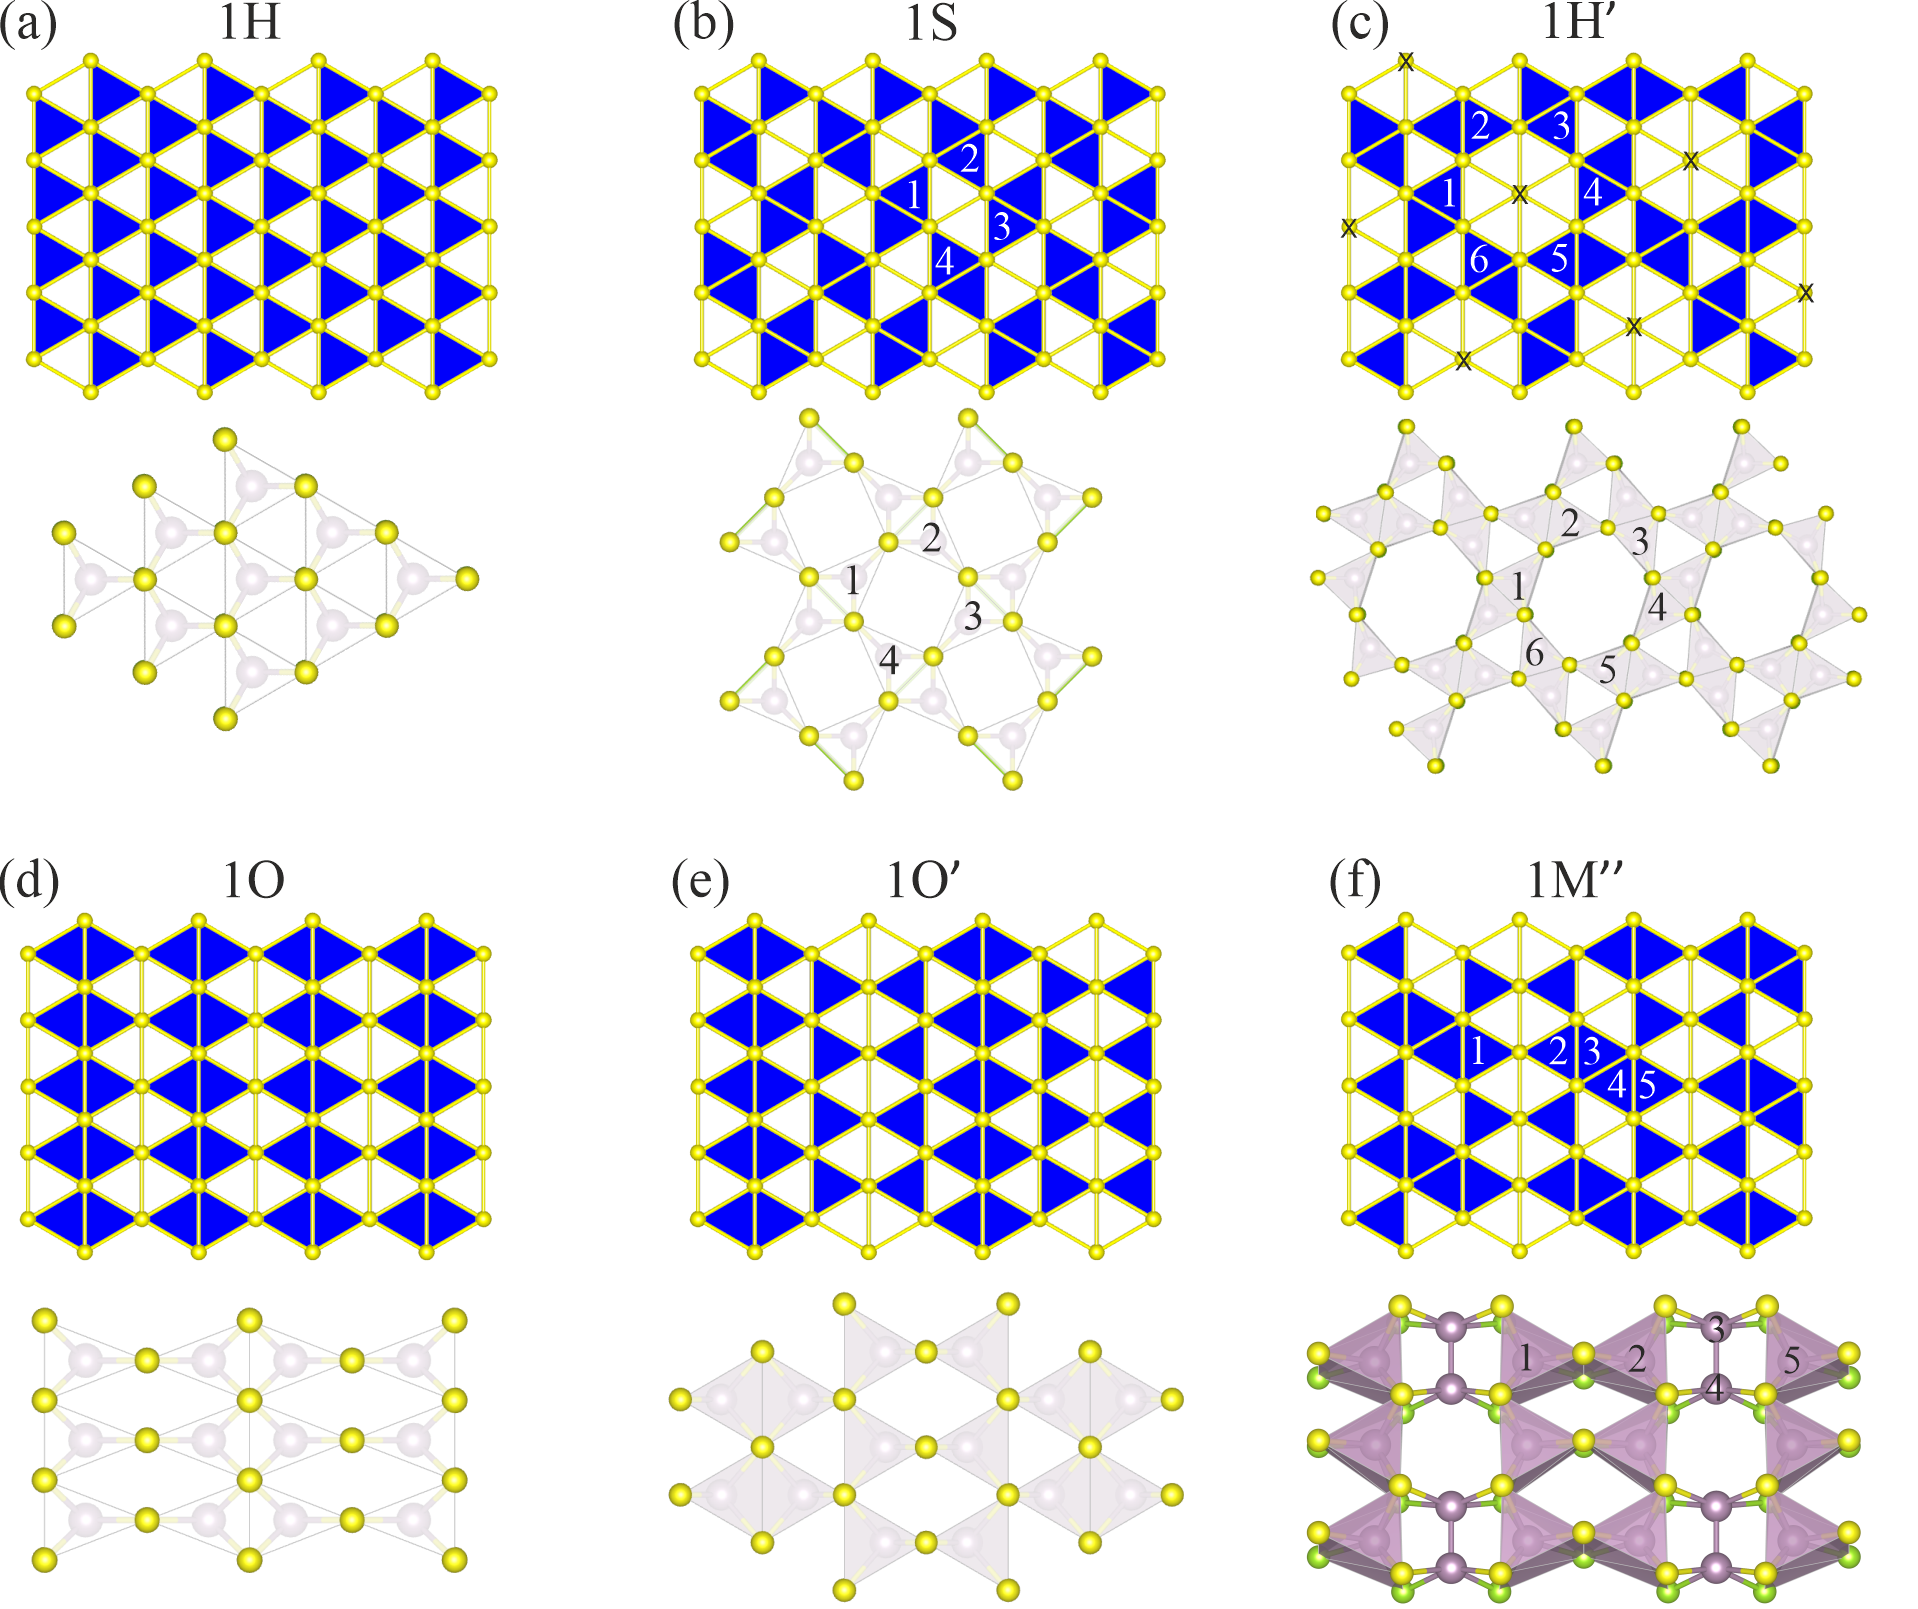
\includegraphics[width=\textwidth]{H-based.png}
        \caption{The initial and optimized structures of SMoSe. Numbers on polyhedra are given to show the same fragment before and after the optimisation.}
\label{H-based}
\end{figure}

\begin{figure}[H]
	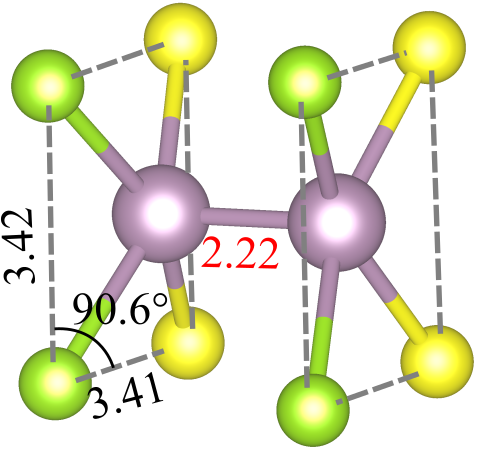
\includegraphics[width=0.3\textwidth]{test3_momo.png}
	\caption{Qadruple Mo--Mo bond in 1M''-SMoSe structure}
\label{test3_momo}
\end{figure}








%%%%%%%%%%%%%%%%%%%%%%%%
\subsection{The uniquenes of the found structures}
%%%%%%%%%%%%%%%%%%%%%%%

To answer the question, whether the found structures are unique or there are similar representatives in ICSD we have performed topological.
The obtained results have shown that all the found structures, except of H-hor, are unique and similar structures are not found in ICSD.
The same is true about the earlier known 1H' and 1S structures, similar structures of which have not also been found. 
The H-hor structure belong to the same kgd topological type as the T structure.
This means that one structure can be transformed into another without breaking the bonds.
However the geometrical difference of H-hor and T structures is sufficient and transformation of one structure into the other requires changing of the coordination polyhedron from trigonal prism to octahedron.

To evaluate the probability for the synthesis of 1A and 1A' structures on the substrate of the other compounds, we have performed the search through the ICSD for the structures with kagome lattices of vanadium or molybdenum atoms.
As the result, 17 structures structures containing flat kagome lattice of vanadium atoms and no structures with flat lattice of of molybdenum atoms have been found. 
The lengths of V--V bonds in the revealed structures vary in the range 2.43--2.81 \AA.
This is close to the lengths of bonds in the mentioned triangular clusters of Mo atoms and sufficiently higher than the lengths of V--V bonds in kagome net of 1A-SVSe.
Thus, based on the structures presented in ICSD it is problematic to suggest the proper substrate for the synthesis of 1A or 1A' structures.




It is worth noting, that ICSD is mainly the databse of experimentally syntheized 3D structures and there can be the structures synthesized in the form of monolayers or theoretically predicted structures which were not included in it.



\subsection{Possible physical properties of the predicted structres}

As it was mentioned above, the special manuscript will be devoted to the calculations of physical properties of the predicted structures.
Here, we would like only to speculate about the possibility of practical applications of the found structures.

The crystal field theory proceeds from the fact that the nature of ligands and their location around the central ion (symmetry of the complex) reduce the degeneracy of $d$-orbitals and change their energy. As all investigated structures consist of TM atoms surrounded by ligands (chalcogen atoms), the presence of the ligands splits the $d$-electrons levels depending on local symmetry. Thereby the correlation between structure and electronic properties can be interpreted in terms of crystal field theory. According to crystal field theory, in an octahedral environment (1T polymorph), the $d$-shell splits into a low-energy triplet (t2g) and a high-energy doublet (eg). In a trigonal prismatic geometry (1H), the low-energy triplet further splits into a doublet and a singlet [https://doi.org/10.1088/2053-1583/ab0188]. The two polymorphs of MoS$_2$ have distinct electronic properties, the 1H-MoS$_2$ is a semiconductor and the 1T-MoS$_2$ is metallic. The 1S-SMoSe despite the prismatic environment of TM atoms becomes a semi-metal [10.1016/j.physe.2020.114485 , 10.1039/D1NA00112D] and Mo- and W-based 1H' structures are gapless semiconductors or, alternatively, semimetals [10.1103/PhysRevB.93.035442]. The proposed structure airss-1 is characterized by a distorted trigonal bipyramidal local environment of the TM atom, which should make this structure more metallic due to degenerated $d$-orbitals. The square-pyramidal environment in airss-3 with the {\bf bare square facet} suggest the possibility for the application of this structure for molecular sorption.
\textcolor{red}{This makes materials based on these structure perspective for sensoric and catalytic uses. In addition, despite the fact that the coordination of metal atoms have a prismatic environment in the geometries 1H' and 1S make metal atoms available for use in chemical applications due to the steric factor. Смысл не ясен}

The variation of structures dictates variation of electronic properties based on different $d$-splitting and electron filling of $d$-orbitals which makes it possible to manipulate electronic properties through phase transformation.
\textcolor{blue}{Захар, надо переделать и добавить 1-2 предложения, т.к. не понятно как последнее предложение соотносится со всем текстом + последнее предложение должно быть завершающим, а тут внезапный обрыв.}


\bibliography{2d}
\bibliographystyle{CGD}


\end{document}


Comment. 
fes structure denoted as S-MS2 in \cite{tang2021_smose}.
fxt structure denoted as H' in \cite{ma2016_h'}.
Similarly there is T' – deformed T-phase.
We can follow this notation, designating our phases by symmetry with addition of '.


2.43--2.56 -- Ta2V3Si
2.81475		-- CaV3Sb4
2.74090		--KV3Sb5
2.53143		--CoVZr
2.61895		-- Vanadium \cite{vanadium}
2.72019		-- molybdenum \cite{molybdenum}

In H-hor structure, atoms of transition metal is in trigonal prismatic coordination, similarly to 1Н structure.
The difference between 1H and H-hor structures is in that in H-hor three-folld symmetry axis of trigonal prism is parallell to the plane of the layer, while in 1H it is perpendicular.

T-hor structure is characterized by the uniqe topology– 3,3,5,8-coordinated net if short V--V bonds are considered and 3,3,5,6-coordinated net if V--V bonds are not considered.
We have not found analogues of these nets in ICSD.

among which are Ta$_2$V$_3$Si \cite{Ta2V3Si}, CaV$_3$Sb$_4$ \cite{ CaV3Sb4}, KV$_3$Sb$_5$ \cite{KV3Sb5}, and CoVZr \cite{ZrVCO}.
The structures with kagome lattice of molybdenum have not been revealed.
The structures of pure vanadium or molybdenum are characterized by the similar bond lengths, which are equal to 2.62 \AA\ \cite{MoV} and 2.72 \AA\ \cite{MoV}, respectively.